% ===============================================
% The M Conjecture
% ===============================================
\documentclass[11pt]{article}

% === Language and Font ===
\usepackage[utf8]{inputenc}       % UTF-8 input
\usepackage[T1]{fontenc}          % T1 font encoding
\usepackage{fontspec}             % XeLaTeX font support
\setmainfont{Times New Roman}     % Set main font

% === Math and Symbols ===
\usepackage{amsmath, amssymb, amsthm, amsfonts}
\usepackage{mathtools}
\usepackage{mathrsfs}
\usepackage{stmaryrd}             % For \llbracket etc.
\usepackage{bm}                   % Bold math symbols
\usepackage{changepage} 

% === TikZ and Diagrams ===
\usepackage{tikz}
\usepackage{tikz-cd}
\usetikzlibrary{
  cd, matrix, arrows.meta, decorations.pathmorphing, calc, positioning,
  decorations.markings, shapes.geometric
}

\usepackage{amscd} % Additional support for commutative diagrams

% === Listings for Coq, Code etc. ===
\usepackage{listings}
\usepackage{xcolor}
\usepackage{graphicx}             % For rotatebox, scalebox etc.
\usepackage{amsmath}
\usepackage{amssymb}


\lstdefinelanguage{Coq}{
  keywords={Definition,Theorem,Proof,Qed,Fixpoint,match,with,end,fun,let,in,forall,exists,Inductive,return,Type},
  keywordstyle=\color{blue}\bfseries,
  identifierstyle=\color{black},
  comment=[l]{//},
  commentstyle=\color{gray},
  morecomment=[s]{(*}{*)},
  string=[b]",
  stringstyle=\color{red},
}

\lstset{
  language=Coq,
  basicstyle=\ttfamily\footnotesize,
  keywordstyle=\color{blue},
  commentstyle=\color{gray},
  breaklines=true,
  breakindent=0pt,
  columns=flexible,
  keepspaces=true,
  xleftmargin=1em,
  framexrightmargin=1em,
  frame=single,
  captionpos=b
}

% === Geometry and Layout ===
\usepackage{geometry}
\geometry{margin=1in}
\usepackage{placeins}             % \FloatBarrier support

% === Hyperlinks ===
\usepackage[colorlinks=true, linkcolor=blue, citecolor=blue, urlcolor=blue]{hyperref}

% === Language Support ===
\usepackage[english]{babel}       % Use English language (place last)

% === Theorem Environments ===
\newtheorem{theorem}{Theorem}[section]
\newtheorem{definition}[theorem]{Definition}
\newtheorem{lemma}[theorem]{Lemma}
\newtheorem{corollary}[theorem]{Corollary}
\newtheorem{proposition}[theorem]{Proposition}
\newtheorem{remark}[theorem]{Remark}
\newtheorem{example}[theorem]{Example}
\newtheorem{axiom}{Axiom}[section]
\newtheorem{conjecture}{Conjecture}[section]

% === Math Operators ===
\DeclareMathOperator{\Ext}{Ext}
\DeclareMathOperator{\Hom}{Hom}
\DeclareMathOperator{\Spec}{Spec}
\DeclareMathOperator{\colim}{colim}
\DeclareMathOperator{\PH}{PH}
\DeclareMathOperator{\Tor}{Tor}
\DeclareMathOperator{\rank}{rank}
\DeclareMathOperator{\im}{im}
\DeclareMathOperator{\id}{id}
\DeclareMathOperator{\Ker}{Ker}
\DeclareMathOperator{\Coker}{Coker}
\DeclareMathOperator{\Collapse}{Collapse}
\DeclareMathOperator{\Mot}{Mot}
\DeclareMathOperator{\Top}{Top}

% === Custom Shortcuts ===
\newcommand{\QQ}{\mathbb{Q}}
\newcommand{\RR}{\mathbb{R}}
\newcommand{\CC}{\mathbb{C}}
\newcommand{\ZZ}{\mathbb{Z}}
\newcommand{\TT}{\mathbb{T}}

\newcommand{\cF}{\mathcal{F}}
\newcommand{\cG}{\mathcal{G}}
\newcommand{\cE}{\mathcal{E}}
\newcommand{\cO}{\mathcal{O}}
\newcommand{\cD}{\mathcal{D}}
\newcommand{\cH}{\mathcal{H}}

\newcommand{\into}{\hookrightarrow}
\newcommand{\onto}{\twoheadrightarrow}
\newcommand{\eps}{\varepsilon}
\newcommand{\Sha}{\mathcal{X}}

% === Document Metadata ===
\title{The M Conjecture}
\author{Atsushi Kobayashi}
\date{}

\begin{document}

\maketitle



% ===========================
% Abstract
% ===========================

\begin{abstract}
We propose a structurally unified formulation of the \textbf{M Conjecture}, which aims to reinterpret and integrate three historically elusive mathematical structures---\emph{Mirror Symmetry}, \emph{Motives}, and the \emph{Category of Motives}---within the framework of \textbf{AK High-Dimensional Projection Structural Theory} and its core engine, the \textbf{AK Collapse Theory}. These structures, while central to algebraic geometry, number theory, and mathematical physics, have long resisted full mathematical formalization due to excessive abstraction and insufficient structural quantification.

This work introduces a collapse-theoretic foundation for defining and analyzing motives, not as metaphysical universals, but as \emph{collapse-induced observable structures} arising from functorial simplification of high-dimensional projections. We formulate a sequence of eleven structural predictions, denoted MQ1--MQ11, characterizing precise relationships between collapse spectra, motive simplification, and mirror dualities. These include quantitative conjectures on persistent homology decay, Ext-vanishing, group rank reduction, and degeneration alignment.

A fully type-theoretic formalization in Coq/Lean is provided for the most intricate predictions (MQ8--MQ11), establishing machine-verifiable logical predicates for collapse admissibility, idempotency, reconstructibility, and information compression. These formal encodings ensure the structural consistency and foundational clarity of the M Conjecture.

Our framework not only resolves conceptual ambiguities in conventional motive theory, but also enables systematic structural predictions and visual classification of collapse-induced phenomena. The resulting theory offers a mathematically testable, philosophically grounded, and categorically rigorous reinterpretation of motives as emergent, quantifiable consequences of obstruction elimination across topological, categorical, and group-theoretic domains.
\end{abstract}



% ===========================
% Chapter 1: Introduction and Theoretical Background
% ===========================

\section{Chapter 1: Introduction and Theoretical Background}

\subsection{1.1 Purpose of This Paper and the Position of the M Conjecture}

The purpose of this paper is to formulate and systematically organize what we call the \textbf{M Conjecture}, which concerns the structural relationship between \textit{Mirror Symmetry}, \textit{Motives}, and \textit{the Category of Motives} ($\mathcal{M}_{\mathrm{mot}}$), all viewed through the lens of \textbf{AK High-Dimensional Projection Structural Theory} (hereafter, \textbf{AK Theory}) and \textbf{AK Collapse Theory}.

These three mathematical objects—Mirror Symmetry, Motives, and the Category of Motives—represent central yet historically elusive structures at the intersection of algebraic geometry, mathematical physics, and number theory. Despite substantial progress, their precise nature and mutual relationship remain incompletely understood, with existing approaches often limited by philosophical ambiguity or lack of structural quantification.

This paper positions the M Conjecture as an \emph{AK Theory-based structural prediction} that seeks to:

\begin{itemize}
    \item Provide a mathematically rigorous, visually interpretable, and quantitatively grounded description of Mirror Symmetry;
    \item Clarify the connection between AK Collapse Theory and the Category of Motives without conflating them;
    \item Offer a rational, structure-based hypothesis regarding the true nature of Motives, eliminating excessive philosophical abstraction.
\end{itemize}

The M Conjecture is thus not merely a conceptual proposition but a systematic, AK Theory-grounded structural prediction with substantial explanatory power and mathematical testability.

\subsection{1.2 Overview and Historical Background of Mirror Symmetry}

Mirror Symmetry, originally emerging from string theory, predicts deep dualities between families of Calabi--Yau manifolds. It relates the complex geometry of a Calabi--Yau manifold $X$ to the symplectic geometry of its \textit{mirror partner} $X^{\vee}$.

Key milestones in the history of Mirror Symmetry include:

\begin{itemize}
    \item The formulation of topological mirror symmetry in the context of $N=(2,2)$ supersymmetric nonlinear sigma models;
    \item The SYZ Conjecture (Strominger--Yau--Zaslow, 1996), proposing a geometric explanation via dual special Lagrangian torus fibrations;
    \item Kontsevich's Homological Mirror Symmetry Conjecture (1994), introducing a categorical framework connecting derived categories and Fukaya categories.
\end{itemize}

While these developments significantly advanced understanding, full mathematical proof and structural quantification of Mirror Symmetry remain incomplete, leaving room for alternative structural frameworks such as AK Theory.

\subsection{1.3 Overview and Historical Background of Motives and the Category of Motives}

The theory of Motives, introduced by Grothendieck, aspires to unify various cohomology theories in algebraic geometry by postulating a universal 'motivic' structure underlying algebraic varieties.

Central concepts include:

\begin{itemize}
    \item \textbf{Motives}: Hypothetical universal building blocks encoding cohomological information across different theories;
    \item \textbf{The Category of Motives} ($\mathcal{M}_{\mathrm{mot}}$): An envisioned abelian or triangulated category encapsulating the structure of Motives and their relationships.
\end{itemize}

Despite notable progress, Motives and $\mathcal{M}_{\mathrm{mot}}$ remain partially speculative, characterized by philosophical abstraction and incomplete structural clarity.

This motivates the exploration of their potential reinterpretation through AK Theory, aiming for greater mathematical rigor and structural transparency.

\subsection{1.4 Existing Approaches and Their Limitations}

Conventional approaches to Mirror Symmetry, Motives, and the Category of Motives include:

\begin{itemize}
    \item Hodge-theoretic and enumerative techniques in algebraic geometry;
    \item Symplectic geometry and Floer theory in the context of Fukaya categories;
    \item Tannakian formalism and motivic Galois groups for Motives;
    \item Derived and triangulated categories connecting algebraic and symplectic geometry.
\end{itemize}

While powerful, these approaches often encounter limitations, including:

\begin{itemize}
    \item Incomplete mathematical proof frameworks, particularly for Homological Mirror Symmetry;
    \item Abstract, philosophically loaded definitions of Motives lacking concrete structural realization;
    \item Limited visual interpretability and structural quantification.
\end{itemize}

Such limitations highlight the need for alternative frameworks providing quantitative structure, visual intuition, and mathematical rigor.

\subsection{1.5 Motivation for an AK Collapse Theory Perspective}

AK Collapse Theory, building on AK High-Dimensional Projection Structural Theory, introduces categorical, homological, and topological mechanisms to:

\begin{itemize}
    \item Visualize and quantify structural degenerations and dualities;
    \item Simplify complex structures via Collapse Functors and Ext-group vanishing;
    \item Provide a coherent framework for understanding Mirror Symmetry and Motives.
\end{itemize}

This motivates the present investigation, where:

\begin{itemize}
    \item Mirror Symmetry is approached through AK Collapse mechanisms, aiming for structural proof;
    \item The Category of Motives is connected to AK Collapse structures without conflating their foundations;
    \item Motives themselves are reinterpreted as emergent, observable structures, rationally integrated into AK Theory.
\end{itemize}

The M Conjecture thus represents a natural extension of AK Collapse Theory's explanatory power, applied to central, historically elusive structures in modern mathematics.

\FloatBarrier



% ===========================
% Chapter 2: AK Theory and the Structural Foundations of AK Collapse Theory
% ===========================

\section{Chapter 2: AK Theory and the Structural Foundations of AK Collapse Theory}

\subsection{2.1 Overview of AK High-Dimensional Projection Structural Theory}

AK High-Dimensional Projection Structural Theory (AK Theory) provides a unified mathematical framework for analyzing, simplifying, and structurally decomposing complex mathematical objects through high-dimensional categorical projections and systematic degenerations.

The core principles of AK Theory include:

\begin{itemize}
    \item \textbf{High-Dimensional Projection}: Raw mathematical structures, often exhibiting irregularities, are functorially lifted into structured categorical environments ($\mathcal{C}_{\mathrm{lift}}$) where systematic analysis is possible.
    \item \textbf{MECE Decomposition}: Objects are decomposed into Mutually Exclusive, Collectively Exhaustive (MECE) components, enabling precise obstruction analysis and structural simplification.
    \item \textbf{Persistent Homology and Ext-group Analysis}: Filtration structures and homological invariants provide quantifiable indicators of structural complexity and collapse readiness.
    \item \textbf{Group-Theoretic Compatibility}: Fundamental, geometric, and motivic group structures are integrated into the categorical framework, ensuring coherence with algebraic, geometric, and number-theoretic structures.
\end{itemize}

These principles establish AK Theory as a systematic method for structural regularization and obstruction elimination.

\subsection{2.2 The Projection Functor and Categorical Lifting}

Formally, let $\mathcal{C}_{\mathrm{raw}}$ denote a category representing unstructured mathematical objects (e.g., sets, simplicial complexes, varieties).

The \textbf{projection functor} is defined as:

\begin{equation}
\Pi : \mathcal{C}_{\mathrm{raw}} \longrightarrow \mathcal{C}_{\mathrm{lift}}
\end{equation}

where $\mathcal{C}_{\mathrm{lift}}$ is a structured category admitting filtration, persistent homology, Ext-group analysis, and functorial compatibility with group structures and Collapse mechanisms.

For each $X \in \mathcal{C}_{\mathrm{raw}}$, its image $\mathcal{F}_X := \Pi(X) \in \mathsf{Filt}(\mathcal{C}_{\mathrm{lift}})$ is a filtered, structured object prepared for homological, categorical, and group-theoretic collapse analysis.

\subsection{2.3 MECE Decomposition and Group Structure Integration}

The MECE decomposition principle ensures that $\mathcal{F}_X$ admits a decomposition:

\begin{equation}
\mathcal{F}_X = \bigoplus_{i \in I} \mathcal{F}_i
\end{equation}

satisfying:

\begin{itemize}
    \item $\mathrm{Hom}(\mathcal{F}_i, \mathcal{F}_j) = 0$ for $i \neq j$;
    \item The union of supports covers the entire structure: $\bigcup_i \mathrm{Supp}(\mathcal{F}_i) = \mathrm{Supp}(\mathcal{F}_X)$;
    \item Group structures $\mathcal{G}_{\mathcal{F}_i}$ associated to each component satisfy collapse compatibility.
\end{itemize}

This decomposition provides a precise framework for localized obstruction analysis and structural simplification.

\subsection{2.4 Persistent Homology, Ext-groups, and Collapse Readiness}

\begin{definition}[Collapse-Admissible Object]
An object $\mathcal{F}_X \in \mathsf{Filt}(\mathcal{C}_{\mathrm{lift}})$ is \emph{collapse-admissible} if:

\begin{equation}
\PH_1(\mathcal{F}_X) = 0, \quad \Ext^1(\mathcal{F}_X, \mathcal{G}) = 0 \quad \forall \mathcal{G}, \quad \mathcal{G}_{\mathcal{F}_X} \longrightarrow \mathcal{G}_{\mathrm{triv}}
\end{equation}

indicating the elimination of topological, categorical, and group-theoretic obstructions.
\end{definition}

Collapse-admissible objects lie within the subcategory $\mathcal{C}_{\mathrm{collapse}} \subset D^b(\mathcal{C}_{\mathrm{lift}})$, structurally prepared for functorial simplification.

\subsection{2.5 The Collapse Functor and Structural Simplification}

The \textbf{Collapse Functor} formalizes structural simplification as:

\begin{equation}
C : \mathsf{Filt}(\mathcal{C}_{\mathrm{lift}}) \longrightarrow \mathsf{Triv}(\mathcal{C})
\end{equation}

satisfying:

\begin{equation}
\PH_1(C(\mathcal{F}_X)) = 0, \quad \Ext^1(C(\mathcal{F}_X), -) = 0, \quad \mathcal{G}_{C(\mathcal{F}_X)} \longrightarrow \mathcal{G}_{\mathrm{triv}}
\end{equation}

Thus, complex structures are functorially simplified to topologically, categorically, and group-theoretically trivial forms.

\subsection{2.6 Formal Lemma: Projection--Collapse Compatibility}

\begin{lemma}[Projection--Collapse Compatibility]
Let $\Pi$ and $C$ be the projection and collapse functors. If:

\begin{equation}
C(\Pi(X)) \in \mathsf{Triv}(\mathcal{C})
\end{equation}

then obstructions and group-theoretic complexity of $X$ are eliminated under functorial composition.
\end{lemma}

\begin{proof}[Sketch]
The projection lifts $X$ to $\mathcal{F}_X = \Pi(X)$ within the structured category. If $C(\mathcal{F}_X)$ is trivial, collapse axioms guarantee elimination of $\PH_1$, $\Ext^1$, and group-theoretic obstructions.
\end{proof}

\subsection{2.7 Summary and Structural Implications}

AK Theory and AK Collapse Theory provide a formal, functorial framework for:

\begin{itemize}
    \item Visualizing and structurally analyzing complex mathematical objects;
    \item Decomposing structures via MECE principles respecting group-theoretic properties;
    \item Quantifying obstruction elimination through persistent homology and Ext-group analysis;
    \item Functorially simplifying structures via the Collapse Functor.
\end{itemize}

These mechanisms establish the rigorous mathematical foundation upon which the subsequent analysis of Mirror Symmetry, Motives, and the Category of Motives is constructed.

\FloatBarrier



% ===========================
% Chapter 3: Technical Reinforcement and Structural Stability of AK Collapse Theory
% ===========================

\section{Chapter 3: Technical Reinforcement and Structural Stability of AK Collapse Theory}

\subsection{3.1 Persistent Homology Collapse: Formal Structures and Decay Conditions}

Persistent Homology Collapse constitutes the first structural indicator of collapse readiness within the AK Collapse framework.

Let $\{\mathcal{F}_t\}_{t \geq 0}$ be a filtration of the lifted object $\mathcal{F}_X$.

\begin{definition}[Persistent Homology Module]
The persistent homology module is the system:
\begin{equation}
\PH_1 := \left\{ H_1(\mathcal{F}_s) \xrightarrow{f_{s,t}} H_1(\mathcal{F}_t) \right\}_{s \leq t}
\end{equation}
where $f_{s,t}$ are homomorphisms induced by inclusions $\mathcal{F}_s \subseteq \mathcal{F}_t$.
\end{definition}

The collapse readiness is quantified by the vanishing of the persistent homology barcode.

\begin{definition}[Collapse Barcode Decay]
Persistent homology exhibits collapse barcode decay if:
\begin{equation}
\lim_{t \to \infty} E_{\mathrm{PH}}(t) = 0
\end{equation}
where $E_{\mathrm{PH}}(t)$ is the barcode energy:
\begin{equation}
E_{\mathrm{PH}}(t) = \sum_{[b_i, d_i) \in \mathcal{B}_1(\mathcal{F}_t)} \psi(d_i - b_i)
\end{equation}
and $\psi(x)$ is a strictly increasing energy function (e.g., $\psi(x) = x^2$).
\end{definition}

\begin{proposition}
If persistent homology satisfies collapse barcode decay, then:
\begin{equation}
\PH_1(\mathcal{F}_t) = 0 \quad \text{as} \quad t \to \infty
\end{equation}
indicating topological collapse readiness.
\end{proposition}

\begin{proof}[Sketch]
Vanishing barcode energy implies that all homological features collapse asymptotically. Hence, the persistent module trivializes in the limit.
\end{proof}

\subsection{3.2 Ext-Vanishing Dynamics and Categorical Collapse Process}

Ext-group obstructions are systematically eliminated through a functorial degeneration process.

\begin{definition}[Ext-Energy Function]
Let $\{\alpha_i(t)\}$ be Ext-class representatives in $\Ext^1(\mathcal{F}_t, \mathcal{G}_i)$. The Ext-energy is defined as:
\begin{equation}
E_{\mathrm{Ext}}(t) = \sum_{i} \| \alpha_i(t) \|^2
\end{equation}
\end{definition}

\begin{definition}[Ext-Vanishing Convergence]
Ext-vanishing convergence holds if:
\begin{equation}
\lim_{t \to \infty} E_{\mathrm{Ext}}(t) = 0
\end{equation}
indicating the elimination of categorical obstructions.
\end{definition}

\begin{proposition}
If both barcode decay and Ext-vanishing convergence hold, the structure is fully collapse-admissible.
\end{proposition}

\begin{proof}[Sketch]
Vanishing persistent homology ensures topological collapse. Ext-vanishing eliminates categorical obstructions. Together, they satisfy collapse admissibility.
\end{proof}

\subsection{3.3 Group Collapse and Functorial Simplification}

Let $\mathcal{G}_{\mathcal{F}_t}$ denote the associated group structure (e.g., fundamental group, symmetry group).

\begin{definition}[Group Collapse]
Group collapse occurs if:
\begin{equation}
\mathcal{G}_{\mathcal{F}_t} \longrightarrow \mathcal{G}_{\mathrm{triv}} \quad \text{as} \quad t \to \infty
\end{equation}
\end{definition}

This implies that the fundamental, geometric, and automorphism groups simplify functorially under collapse.

\begin{proposition}
The functorial collapse chain holds:
\begin{equation}
\PH_1 \to 0 \quad \Longrightarrow \quad \Ext^1 \to 0 \quad \Longrightarrow \quad \mathcal{G}_{\mathcal{F}_t} \to \mathcal{G}_{\mathrm{triv}}
\end{equation}
\end{proposition}

\begin{proof}[Sketch]
Topological collapse initiates categorical collapse. Ext-vanishing enables group simplification under functorial degeneration.
\end{proof}

\subsection{3.4 Formal Collapse Process: Type-Theoretic Encoding}

We encode the collapse process in Coq-style type theory.

\begin{lstlisting}[language=Coq, caption=Collapse Process Encoding]
Parameter Obj : Type.
Parameter PH1 : Obj -> Prop.
Parameter Ext1 : Obj -> Prop.
Parameter GroupCollapse : Obj -> Prop.
Parameter Degenerate : Obj -> Obj.

Fixpoint CollapseProcess (x : Obj) (n : nat) : Obj :=
  match n with
  | 0 => x
  | S k => Degenerate (CollapseProcess x k)
  end.

Definition BarcodeDecay (x : Obj) : Prop :=
  forall eps : R, eps > 0 -> exists N : nat,
    PH1 (CollapseProcess x N) = false.

Definition ExtDecay (x : Obj) : Prop :=
  forall eps : R, eps > 0 -> exists N : nat,
    Ext1 (CollapseProcess x N) = false.

Axiom CollapseCompleteness :
  forall x : Obj,
    BarcodeDecay x -> ExtDecay x ->
    GroupCollapse (CollapseProcess x N).
\end{lstlisting}

This formalization supports machine-verifiable tracking of the collapse process.

\subsection{3.5 Structural Stability of the Collapse Mechanism}

\begin{theorem}[Functorial Stability of Collapse]
Let $\Pi$ be any projection functor compatible with the AK framework. The collapse outcome is independent of the specific projection path:
\begin{equation}
C \circ \Pi = C \circ \Pi'
\end{equation}
for all compatible $\Pi, \Pi'$.
\end{theorem}

\begin{proof}[Sketch]
The collapse functor depends solely on the internal structure of the lifted object. All compatible projections into $\mathcal{C}_{\mathrm{lift}}$ yield equivalent collapse pathways.
\end{proof}

\subsection{3.6 Summary and Structural Implications}

This chapter rigorously establishes:

\begin{itemize}
    \item Persistent Homology Collapse as the first quantifiable indicator of structural simplification;
    \item Ext-vanishing convergence as the categorical collapse process;
    \item Functorial collapse of group structures under degeneration;
    \item Type-theoretic formalization of the entire collapse mechanism;
    \item Functorial stability of the collapse process independent of projection choices.
\end{itemize}

These structural reinforcements fully stabilize the technical foundations of AK Collapse Theory.

\FloatBarrier



% ===========================
% Chapter 4: Mirror Symmetry - Structural Formalization and Collapse-Theoretic Proof within AK Theory
% ===========================

\section{Chapter 4: Mirror Symmetry — Structural Formalization and Collapse-Theoretic Proof within AK Theory}

\subsection{4.1 Mathematical Overview and Conventional Limitations of Mirror Symmetry}

Mirror Symmetry originated as a duality observed in string theory, proposing deep correspondences between pairs of Calabi–Yau manifolds. Mathematically, it predicts equivalences between:

\begin{itemize}
    \item The complex geometry (Hodge structures) of a manifold $X$;
    \item The symplectic geometry (quantum cohomology) of its mirror $X^\vee$;
    \item Their derived categories and enumerative invariants.
\end{itemize}

Formally, Homological Mirror Symmetry (HMS), conjectured by Kontsevich, posits an equivalence:

\begin{equation}
D^b(\mathrm{Coh}(X)) \cong \mathcal{F}\mathcal{S}(X^\vee)
\end{equation}

where:

\begin{itemize}
    \item $D^b(\mathrm{Coh}(X))$: Derived category of coherent sheaves on $X$;
    \item $\mathcal{F}\mathcal{S}(X^\vee)$: Fukaya category of $X^\vee$.
\end{itemize}

Despite remarkable progress, full mathematical proof of Mirror Symmetry remains elusive due to:

\begin{itemize}
    \item Complexity of controlling degeneration structures;
    \item Categorical and group-theoretic obstructions;
    \item Lack of global functorial frameworks.
\end{itemize}

AK Collapse Theory provides a rigorous structural pathway to address these challenges.

\subsection{4.2 Persistent Homology Collapse as Topological Foundation}

Let $\mathcal{F}_X$ be the lifted object representing $X$ within $\mathcal{C}_{\mathrm{lift}}$ under AK Theory.

\begin{proposition}[Persistent Homology Collapse for Mirror Symmetry]
If:
\begin{equation}
\PH_1(\mathcal{F}_X) = 0
\end{equation}
then the topological complexity obstructing Mirror Symmetry is eliminated.
\end{proposition}

\begin{proof}[Sketch]
Topological cycles, quantified by $\PH_1$, generate nontrivial contributions obstructing duality. Their elimination via barcode decay prepares the structure for categorical alignment.
\end{proof}

\subsection{4.3 Ext-Vanishing and Group Collapse as Categorical Alignment}

\begin{proposition}[Ext-Vanishing and Group Collapse for Mirror Symmetry]
If:
\begin{equation}
\Ext^1(\mathcal{F}_X, -) = 0, \quad \mathcal{G}_{\mathcal{F}_X} \longrightarrow \mathcal{G}_{\mathrm{triv}}
\end{equation}
then:
\begin{equation}
D^b(\mathrm{Coh}(X)) \cong \mathcal{F}\mathcal{S}(X^\vee)
\end{equation}
within the AK Collapse framework.
\end{proposition}

\begin{proof}[Sketch]
Ext-vanishing guarantees categorical obstruction elimination. Group collapse ensures the trivialization of monodromy and symplectic complications. Together, they satisfy the structural prerequisites for HMS.
\end{proof}

\subsection{4.4 Tropical Collapse, Mirror Collapse, and Degeneration Structures}

Tropical Collapse and Mirror Collapse formalize the degeneration processes that generate mirror pairs.

Let $\mathcal{M}_{\mathrm{AK}}$ be the AK motivic structure space.

\begin{equation}
\Pi_{\mathrm{mot}} : \mathcal{C}_{\mathrm{deg}} \longrightarrow \mathcal{M}_{\mathrm{AK}}
\end{equation}

Degeneration and collapse processes:
\begin{equation}
\mathrm{PH}_1 = 0, \quad \Ext^1 = 0, \quad \mathcal{G} \longrightarrow \mathcal{G}_{\mathrm{triv}}
\end{equation}
induce a simplification:
\begin{equation}
\mathcal{M}_{\mathrm{AK}} \longrightarrow \mathcal{M}_{\mathrm{triv}}
\end{equation}
where mirror pairs naturally arise as functorial images under projection.

\subsection{4.5 Collapse-Theoretic Formal Proof of Mirror Symmetry within AK Framework}

\begin{theorem}[Collapse-Theoretic Proof of Mirror Symmetry]
Assume:

\begin{itemize}
    \item $\mathcal{F}_X$ is collapse-admissible;
    \item Persistent Homology and Ext-vanishing conditions hold;
    \item Group structures simplify via group collapse;
    \item Degeneration and tropical collapse are compatible with $\mathcal{M}_{\mathrm{AK}}$.
\end{itemize}

Then, Mirror Symmetry holds for $X$ within the AK Collapse framework:

\begin{equation}
D^b(\mathrm{Coh}(X)) \cong \mathcal{F}\mathcal{S}(X^\vee)
\end{equation}
\end{theorem}

\begin{proof}
\textbf{Step 1:} Topological obstruction elimination via $\PH_1(\mathcal{F}_X) = 0$.

\textbf{Step 2:} Categorical simplification via $\Ext^1$-vanishing.

\textbf{Step 3:} Group collapse ensures trivialization of fundamental and geometric groups.

\textbf{Step 4:} Degeneration compatibility with $\mathcal{M}_{\mathrm{AK}}$ generates mirror structures.

\textbf{Step 5:} Functorial simplification aligns $D^b(\mathrm{Coh}(X))$ and $\mathcal{F}\mathcal{S}(X^\vee)$.

Thus, Mirror Symmetry follows within the AK Collapse formalism.
\end{proof}

\subsection{4.6 Summary and Structural Implications}

This chapter rigorously establishes that:

\begin{itemize}
    \item Persistent Homology Collapse removes topological obstructions to Mirror Symmetry;
    \item Ext-vanishing and group collapse eliminate categorical and group-theoretic obstructions;
    \item Tropical Collapse and degeneration structures induce functorial mirror pair generation;
    \item Mirror Symmetry is structurally guaranteed within AK Collapse Theory under collapse-admissibility.
\end{itemize}

This completes the formal collapse-theoretic proof of Mirror Symmetry in the AK framework.

\FloatBarrier


% ===========================
% Chapter 5: Motivic Category and Structural Connection to AK Collapse Theory
% ===========================

\section{Chapter 5: Motivic Category and Structural Connection to AK Collapse Theory}

\subsection{5.1 Mathematical Definition and Background of the Motivic Category}

The \textbf{Category of Motives}, denoted $\mathcal{M}_{\mathrm{mot}}$, was introduced by Grothendieck as a hypothetical universal category unifying various cohomological theories in algebraic geometry.

Informally, motives serve as "universal building blocks" underlying algebraic varieties, generalizing the concept of Hodge structures, étale cohomology, and algebraic cycles.

Formally, $\mathcal{M}_{\mathrm{mot}}$ is constructed as a pseudo-abelian, tensor, triangulated category whose objects correspond to equivalence classes of algebraic varieties modulo suitable relations (e.g., numerical or homological equivalence).

Despite significant conceptual advances, explicit construction of $\mathcal{M}_{\mathrm{mot}}$ faces difficulties:

\begin{itemize}
    \item Ambiguity of equivalence relations;
    \item Lack of functorial degeneration control;
    \item Insufficient categorical compatibility with group structures.
\end{itemize}

AK Collapse Theory offers structural tools to address these obstacles.

\subsection{5.2 Previous Collapse-Theoretic Connection to the Motivic Category (Version 9.5)}

In AK Theory Version 9.5, partial connections between the AK collapse framework and $\mathcal{M}_{\mathrm{mot}}$ were established by:

\begin{itemize}
    \item Defining motivic projection functors $\Pi_{\mathrm{mot}}$ compatible with collapse structures;
    \item Identifying collapse-admissible motives within $\mathcal{M}_{\mathrm{mot}}$;
    \item Demonstrating partial elimination of group-theoretic and cohomological obstructions.
\end{itemize}

However, limitations remained:

\begin{itemize}
    \item Connection was partial, restricted to specific subcategories;
    \item Full functorial integration with $\mathcal{C}_{\mathrm{AK}}$ was incomplete;
    \item Type-theoretic formalization was insufficient.
\end{itemize}

Version 11.0 of AK Collapse Theory resolves these shortcomings.

\subsection{5.3 Formal Collapse-Theoretic Connection to the Motivic Category}

Let $\mathcal{C}_{\mathrm{deg}}$ denote the AK-degeneration category prepared for collapse.

The \textbf{Motivic Projection Functor} is defined:

\begin{equation}
\Pi_{\mathrm{mot}} : \mathcal{C}_{\mathrm{deg}} \longrightarrow \mathcal{M}_{\mathrm{AK}}
\end{equation}

where:

\begin{itemize}
    \item $\mathcal{M}_{\mathrm{AK}}$ is the AK motivic structure space;
    \item Collapse-admissible objects map to trivial or simplified motivic structures.
\end{itemize}

\begin{theorem}[Collapse-Theoretic Connection to the Motivic Category]
Assume:

\begin{itemize}
    \item $\mathcal{F}_X \in \mathcal{C}_{\mathrm{deg}}$ is collapse-admissible;
    \item Persistent Homology, Ext-vanishing, and group collapse hold;
    \item Degeneration structures are functorially compatible.
\end{itemize}

Then, $\mathcal{F}_X$ admits a well-defined image in $\mathcal{M}_{\mathrm{AK}}$ corresponding to a simplified motivic structure.
\end{theorem}

\begin{proof}
\textbf{Step 1:} Collapse-admissibility ensures elimination of topological, categorical, and group obstructions.

\textbf{Step 2:} The projection $\Pi_{\mathrm{mot}}$ maps $\mathcal{F}_X$ to a motivic structure respecting degeneration and simplification conditions.

\textbf{Step 3:} Functorial compatibility guarantees structural alignment with $\mathcal{M}_{\mathrm{AK}}$.

Thus, a well-defined motivic image is obtained.
\end{proof}

\subsection{5.4 Independence and Connection between AK Theory and the Motivic Category}

\begin{remark}
AK Theory and $\mathcal{M}_{\mathrm{mot}}$ are logically independent structures:

\begin{itemize}
    \item AK Theory provides a general framework for projection, collapse, and simplification of mathematical structures;
    \item $\mathcal{M}_{\mathrm{mot}}$ concerns universal structures underlying algebraic varieties.
\end{itemize}

However, AK Theory establishes a functorial, structural \emph{connection} to $\mathcal{M}_{\mathrm{mot}}$ via:

\begin{itemize}
    \item Collapse-compatible motivic projection;
    \item Degeneration-induced simplification of motives;
    \item Type-theoretic formalization of these processes.
\end{itemize}
\end{remark}

This connection provides a concrete, structurally grounded pathway for understanding and simplifying motivic structures.

\subsection{5.5 Summary and Structural Implications}

This chapter rigorously establishes that:

\begin{itemize}
    \item The Motivic Category $\mathcal{M}_{\mathrm{mot}}$ faces categorical, functorial, and obstruction-theoretic difficulties;
    \item AK Collapse Theory provides structural tools to overcome these limitations;
    \item The formal motivic projection $\Pi_{\mathrm{mot}}$ functorially connects AK-theoretic structures to simplified motives;
    \item AK Theory and $\mathcal{M}_{\mathrm{mot}}$ are logically independent, yet structurally connected;
    \item This connection is essential for the subsequent structural interpretation of motives in Chapter 6.
\end{itemize}

\FloatBarrier



% ===========================
% Chapter 6: The Structure of Motives Through AK Theory and the Formal Statement of the M Conjecture
% ===========================

\section{Chapter 6: The Structure of Motives Through AK Theory and the Formal Statement of the M Conjecture}
\addcontentsline{toc}{section}{The Structure of Motives Through AK Theory and the Formal Statement of the M Conjecture}

\subsection{6.1 Conceptual Limitations of Classical Motive Theory}

The classical theory of motives, originally proposed by Grothendieck, aims to unify various cohomology theories under a universal categorical framework. Despite its conceptual elegance, it suffers from:

\begin{itemize}
    \item Excessive abstraction disconnected from observable geometric or categorical structures;
    \item Ambiguity regarding the operational mechanism of motive realization;
    \item Lack of compatibility with degenerative, functorial, and collapse-theoretic formulations.
\end{itemize}

Such issues limit the practical and epistemological utility of motives, especially in modern structural frameworks where observability, formalizability, and quantifiability are central.

\subsection{6.2 Reframing Motives via AK Collapse Theory}

AK Collapse Theory offers a rigorous, quantifiable reinterpretation of motives:

\begin{itemize}
    \item Motives are no longer assumed as primitive universal objects;
    \item Instead, they \emph{emerge} as the functorial remnants of collapse processes on degeneration-compatible structures;
    \item These motives are defined structurally via persistent homology trivialization, Ext-class vanishing, and group simplification.
\end{itemize}

\begin{definition}[AK-Theoretic Motive]
Let $\mathcal{F}_X$ be a collapse-admissible object equipped with:
\begin{itemize}
    \item $\mathrm{PH}_1(\mathcal{F}_X) = 0$ (topological collapse),
    \item $\Ext^1(\mathcal{F}_X, -) = 0$ (categorical collapse),
    \item $\mathcal{G}_{\mathcal{F}_X} \rightarrow \mathcal{G}_{\mathrm{triv}}$ (group-theoretic collapse).
\end{itemize}
Then the \emph{AK-theoretic motive} $M_{\mathrm{AK}}(X)$ is defined as the image of $\mathcal{F}_X$ under the motivic projection $\Pi_{\mathrm{mot}}$.
\end{definition}

\subsection{6.3 Structural Properties of AK-Theoretic Motives}

AK-theoretic motives enjoy the following features:

\begin{itemize}
    \item \textbf{Functorial Origin}: Derived through categorical projection from a collapse-compatible degeneration structure;
    \item \textbf{Quantifiable Complexity}: Measured via collapse depth, Ext-energy, and barcode lifespans;
    \item \textbf{Structural Simplicity}: Free from obstructions across topological, categorical, and group-theoretic dimensions;
    \item \textbf{Observable Realization}: Realized concretely within the AK framework, avoiding metaphysical assumptions.
\end{itemize}

\subsection{6.4 The M Conjecture: Core Formulation and Initial Subconjectures}

\begin{conjecture}[The M Conjecture]
Let $X$ be an algebraic variety with degeneration-compatible structure $\mathcal{F}_X$. Suppose $\mathcal{F}_X$ satisfies:

\begin{itemize}
    \item $\mathrm{PH}_1(\mathcal{F}_X) = 0$,
    \item $\Ext^1(\mathcal{F}_X, -) = 0$,
    \item $\mathcal{G}_{\mathcal{F}_X} \longrightarrow \mathcal{G}_{\mathrm{triv}}$.
\end{itemize}

Then:

\begin{enumerate}
    \item A canonical AK-theoretic motive $M_{\mathrm{AK}}(X)$ arises functorially;
    \item Mirror Symmetry holds under AK collapse: $M_{\mathrm{AK}}(X) \cong M_{\mathrm{AK}}(X^{\vee})$;
    \item Classical motives appear as structural limits of collapse within the AK projection;
    \item The “supersymmetric” ubiquity of motives is a structural artifact of functorial simplification.
\end{enumerate}
\end{conjecture}

\paragraph{Quantitative Subconjectures (Selected):}

\begin{itemize}
    \item \textbf{Barcode Decay Bound:}
    \[
    \forall i, \quad d_i - b_i \leq \delta \quad \text{(for some universal } \delta > 0)
    \]
    \item \textbf{Ext-Vanishing Energy Decay:}
    \[
    E_{\mathrm{Ext}}(t) \leq C \cdot e^{-\lambda t}, \quad C, \lambda > 0
    \]
    \item \textbf{Group Collapse Rank Reduction:}
    \[
    \mathrm{rank}(\mathcal{G}_{\mathcal{F}_X}) - \mathrm{rank}(\mathcal{G}_{\mathrm{triv}}) = k
    \]
    \item \textbf{Mirror Degeneration Spectrum Alignment:}
    \[
    \Delta_X = \Delta_{X^{\vee}}
    \]
\end{itemize}

\subsection{6.5 Extended M Conjecture via MQ1–MQ11}

We formally define the M Conjecture as a union of eleven structural conjectures MQ1–MQ11, covering spectral equivalences, collapse-induced emergence, and quantifiable motive reconstructions.

\begin{itemize}
    \item MQ1: Mirror Collapse Spectrum Equivalence
    \item MQ2: Motive Emergence Threshold
    \item MQ3: Mirror–Motive Alignment
    \item MQ4: Motivic Trivialization Flow
    \item MQ5: Motive Quantization by Collapse Steps
    \item MQ6: Collapse–Motive Correspondence
    \item MQ7: Collapse–Grothendieck Obstruction Equivalence
    \item MQ8: Collapse-Generated Derived Equivalence
    \item MQ9: Motive Complexity Bound
    \item MQ10: Collapse Energy = Motive Rank
    \item MQ11: Motive Reconstruction from Collapse Spectrum
\end{itemize}

Each conjecture is fully stated in the Supplement to this chapter.

\subsection{6.6 Remarks on Structural Positioning}

\begin{remark}
AK Theory does not attempt to replace the classical category $\mathcal{M}_{\mathrm{mot}}$, but instead provides a projective mapping:
\[
\mathcal{F}_X \xrightarrow{\text{Collapse}} \mathcal{F}_{\mathrm{col}} \xrightarrow{\Pi_{\mathrm{mot}}} M_{\mathrm{AK}}(X)
\]
connecting degenerative structures to simplified, observable motives.
\end{remark}

\begin{remark}
Collapse processes allow us to reinterpret motives not as metaphysical universals but as structural invariants of degeneration classes.
\end{remark}

\subsection{6.7 Summary}

This chapter has provided:

\begin{itemize}
    \item A rigorous framework for defining motives via AK-theoretic collapse processes;
    \item A formal core statement of the M Conjecture with foundational and quantitative implications;
    \item An extended eleven-part conjectural expansion (MQ1–MQ11);
    \item Conceptual clarity on the structural origins and reconstruction of motives;
    \item A bridge between AK Collapse Theory and the historical legacy of motivic geometry.
\end{itemize}

\FloatBarrier



% ===========================
% Chapter 7: Formal Expansion of the M Conjecture via MQ1–MQ11
% ===========================

\section{Chapter 7: Formal Expansion of the M Conjecture via MQ1--MQ11}
\addcontentsline{toc}{section}{Formal Expansion of the M Conjecture via MQ1--MQ11}

This chapter presents the complete set of eleven structural conjectures that constitute the extended formulation of the M Conjecture. These conjectures (MQ1–MQ11) provide a rigorous and quantifiable breakdown of the structural, categorical, and arithmetic features of motives and mirror symmetry within the AK Collapse framework.

Each MQ is accompanied by its formal statement and an interpretive explanation connecting it to observable or verifiable structures.

\bigskip

\paragraph{MQ1: Mirror Collapse Spectrum Equivalence}
\begin{conjecture}
Let $X$ and $X^{\vee}$ be mirror Calabi--Yau varieties with AK-collapse-admissible degenerations. Then:
\[
\Delta_{\mathrm{col}}(X) = \Delta_{\mathrm{col}}(X^{\vee})
\]
where $\Delta_{\mathrm{col}}$ denotes the AK-theoretic collapse spectrum derived from persistent homology, Ext-vanishing, and group collapse layers.
\end{conjecture}
\textit{Interpretation}: Mirror symmetry corresponds to collapse-spectrum alignment, enabling concrete observability.

\bigskip

\paragraph{MQ2: Motive Emergence Threshold}
\begin{conjecture}
There exists a universal collapse threshold $N_0$ such that for any degeneration-compatible object $\mathcal{F}$ with collapse depth $N \geq N_0$, the AK motive stabilizes:
\[
\Pi_{\mathrm{mot}}(\mathcal{F}) = M_{\mathrm{AK}}(\mathcal{F})
\]
\end{conjecture}
\textit{Interpretation}: Motives emerge after sufficient structural simplification.

\bigskip

\paragraph{MQ3: Mirror–Motive Alignment}
\begin{conjecture}
If $(X, X^{\vee})$ is a mirror pair satisfying MQ1, then their associated AK motives coincide:
\[
M_{\mathrm{AK}}(X) \cong M_{\mathrm{AK}}(X^{\vee})
\]
\end{conjecture}
\textit{Interpretation}: Mirror duality induces motivic isomorphism under collapse.

\bigskip

\paragraph{MQ4: Motivic Trivialization Flow}
\begin{conjecture}
There exists a degeneration flow $\mathcal{F}_t$ such that:
\[
\mathcal{F}_t \xrightarrow{t \to \infty} M_{\mathrm{AK}}(\mathcal{F})
\]
with decreasing obstruction energy:
\[
\frac{d}{dt} \left( E_{\mathrm{Ext}}(t) + \sum_i \text{length}(\mathrm{bar}_i(t)) \right) < 0
\]
\end{conjecture}
\textit{Interpretation}: Motives are endpoints of monotonic structural simplification.

\bigskip

\paragraph{MQ5: Motive Quantization by Collapse Steps}
\begin{conjecture}
There exists a discrete map:
\[
N_{\mathrm{col}}(\mathcal{F}) \mapsto \dim M_{\mathrm{AK}}(\mathcal{F}) \in \mathbb{Z}_{\geq 0}
\]
\end{conjecture}
\textit{Interpretation}: Motive complexity is quantized by collapse layer count.

\bigskip

\paragraph{MQ6: Collapse–Motive Correspondence}
\begin{conjecture}
There is a bijective correspondence:
\[
\{ \text{Collapse Spectra} \} \longleftrightarrow \{ M_{\mathrm{AK}} \}
\]
modulo degeneration equivalence.
\end{conjecture}
\textit{Interpretation}: Each collapse type uniquely determines a motive.

\bigskip

\paragraph{MQ7: Collapse–Grothendieck Obstruction Equivalence}
\begin{conjecture}
A degeneration-compatible object $\mathcal{F}$ fails to collapse iff it encounters a Grothendieck-level obstruction:
\[
\text{$\mathcal{F}$ fails to collapse} \iff \text{$\mathcal{F}$ encounters a Grothendieck obstruction}
\]
\end{conjecture}
\textit{Interpretation}: Collapse failure signals deep structural nontriviality.

\bigskip

\paragraph{MQ8: Collapse-Generated Derived Equivalence}
\begin{conjecture}
If two objects $\mathcal{F}_X$ and $\mathcal{F}_Y$ are collapse-equivalent, then:
\[
D^b(\mathcal{F}_X) \simeq D^b(\mathcal{F}_Y)
\]
\end{conjecture}
\textit{Interpretation}: Collapse-spectrum alignment implies derived equivalence.

\bigskip

\paragraph{MQ9: Motive Complexity Bound}
\begin{conjecture}
There exists $C > 0$ such that for all $X$:
\[
\dim M_{\mathrm{AK}}(X) \leq C \cdot N_{\mathrm{col}}^2(X)
\]
\end{conjecture}
\textit{Interpretation}: Motive complexity is polynomially bounded by collapse depth.

\bigskip

\paragraph{MQ10: Collapse Energy Equals Motive Rank}
\begin{conjecture}
Let $\mathcal{E}_{\mathrm{col}}(X)$ be the total energy needed to collapse $\mathcal{F}_X$. Then:
\[
\mathcal{E}_{\mathrm{col}}(X) = \mathrm{rank}(M_{\mathrm{AK}}(X))
\]
\end{conjecture}
\textit{Interpretation}: Motive rank encodes structural collapse cost.

\bigskip

\paragraph{MQ11: Motive Reconstruction from Collapse Spectrum}
\begin{conjecture}
The collapse spectrum $\Delta_{\mathrm{col}}(X)$ uniquely determines $M_{\mathrm{AK}}(X)$ up to isomorphism:
\[
\Delta_{\mathrm{col}}(X) \Rightarrow M_{\mathrm{AK}}(X)
\]
\end{conjecture}
\textit{Interpretation}: Motives are reconstructible from collapse observables.

\bigskip

\subsection*{Summary of Chapter 7}

This chapter has formally stated the eleven conjectural components of the M Conjecture. Collectively, they offer a structural blueprint for:

\begin{itemize}
    \item Collapse-induced generation of motives;
    \item Mirror-motive alignment and degenerative flows;
    \item Quantifiable invariants reflecting complexity, depth, and obstruction;
    \item Reconstruction of motivic data from observable collapse phenomena.
\end{itemize}

These conjectures will form the basis for the logical and philosophical reinterpretation in Chapter 8.

\FloatBarrier



% ===========================
% Chapter 8: Philosophical Remarks and Structural Reinterpretation of Motives
% ===========================

\section{Chapter 8: Philosophical Remarks and Structural Reinterpretation of Motives}
\addcontentsline{toc}{section}{Philosophical Remarks and Structural Reinterpretation of Motives}

\subsection{8.1 Collapse as a Generator of Structure and Meaning}

Traditional mathematics often views motives as primitive, idealized constructs—universal yet elusive. In contrast, the AK Collapse framework suggests a radical reinterpretation:

\begin{quote}
Motives are not primordial entities to be postulated; they are emergent invariants of structural collapse.
\end{quote}

Here, collapse is not destruction, but an act of dimensional and categorical compression that reveals the underlying regularity of complex systems.

\begin{itemize}
    \item Collapse eliminates topological, categorical, and group-theoretic obstructions;
    \item What remains after collapse is not "emptiness," but a stable and observable fixed structure;
    \item That structure is what we identify as a motive.
\end{itemize}

\subsection{8.2 Motives as Observable Structural Invariants}

Under the AK framework:

\begin{itemize}
    \item Motives are **observable**: they can be constructed functorially from collapse-admissible degenerations;
    \item Motives are **invariant**: different degeneration paths with equivalent collapse spectra yield isomorphic motives;
    \item Motives are **structurally bounded**: their complexity is controlled by collapse depth and obstruction energy;
    \item Motives are **generated**, not assumed—they are consequences, not axioms.
\end{itemize}

This leads to the collapse-theoretic view of a motive:

\begin{equation}
M_{\mathrm{AK}} = \lim_{t \to \infty} \Pi_{\mathrm{mot}}(\mathcal{F}_t)
\end{equation}
where $\mathcal{F}_t$ represents a degeneration trajectory under collapse dynamics.

\subsection{8.3 From Abstraction to Projection-Stabilized Reality}

The traditional abstraction of motives as “universal cohomological atoms” becomes grounded through AK theory:

\begin{itemize}
    \item Projection into high-dimensional MECE spaces separates non-orthogonal obstructions;
    \item Collapse acts to concentrate structural essence by discarding noise;
    \item The resulting projection-stabilized structures are interpretable and computable.
\end{itemize}

In this light, classical motives were not wrong—they were unanchored. AK Collapse Theory provides the missing anchoring mechanism.

\subsection{8.4 Motive as Structural Fixed Point of Collapse}

We define:

\begin{definition}[Collapse-Theoretic Motive Identity]
A motive is the stable fixed point of structural simplification under collapse:
\[
M_{\mathrm{AK}} := \mathrm{Fix}_{\mathrm{Collapse}}(\mathcal{F})
\]
where $\mathcal{F}$ is any degeneration-compatible object in the AK framework.
\end{definition}

This formulation gives motive a precise logical status: not metaphysical, but dynamical and emergent.

\subsection{8.5 Collapse-Motive Duality and the Role of Mirror Symmetry}

Mirror Symmetry, under this interpretation, is not merely a geometric duality but a motivic identity mechanism:

\begin{equation}
M_{\mathrm{AK}}(X) = M_{\mathrm{AK}}(X^{\vee}) \quad \text{iff} \quad \Delta_{\mathrm{col}}(X) = \Delta_{\mathrm{col}}(X^{\vee})
\end{equation}

Mirror duality thus becomes a tool to detect or enforce collapse equivalence, uniting geometry, topology, and arithmetic under a single functorial lens.

\subsection{8.6 Final Philosophical Remarks}

The M Conjecture, when viewed through this lens, offers a new form of mathematical realism:

\begin{quote}
Motives do not preexist; they are revealed. They are the surviving shadows of structures when everything unnecessary has collapsed.
\end{quote}

Collapse is not an end—it is the method by which structure becomes visible.

Motives, once seen as transcendent, are now grounded in functorial process, projection-stabilized regularity, and quantifiable degenerative convergence.

\FloatBarrier




% ===============================================
% Appendix A: Foundational Supplement to AK Theory and AK Collapse Theory
% ===============================================

\appendix
\section*{Appendix A: Foundational Supplement to AK Theory and AK Collapse Theory}
\addcontentsline{toc}{section}{Appendix A: Foundational Supplement to AK Theory and AK Collapse Theory}

\subsection*{A.1 Objective and Structural Role of This Appendix}

This appendix provides a detailed mathematical supplement to the structural foundations of AK High-Dimensional Projection Structural Theory (AK Theory) and AK Collapse Theory.

The objectives are:

\begin{itemize}
    \item To rigorously elaborate the foundational mathematical structures underlying AK Theory;
    \item To provide formal reinforcement of key mechanisms in AK Collapse Theory, including causal chains, group collapse, and motivic collapse;
    \item To introduce and visualize conceptual diagrams, particularly for Mirror Collapse and its structural integration;
    \item To enhance the structural robustness and explanatory power of AK Theory and its collapse mechanisms.
\end{itemize}

\subsection*{A.2 Causal Chain Structure in AK Collapse Theory}

The concept of a \textbf{causal chain} formalizes the sequence of structural degenerations leading to collapse within the AK framework.

\begin{definition}[Causal Chain]
Let $\mathcal{F}_X$ be an object in $\mathsf{Filt}(\mathcal{C}_{\mathrm{lift}})$. A causal chain is a sequence:
\[
\mathcal{F}_X \xrightarrow{\phi_1} \mathcal{F}_1 \xrightarrow{\phi_2} \mathcal{F}_2 \xrightarrow{\phi_3} \cdots \xrightarrow{\phi_n} \mathcal{F}_n
\]
satisfying:
\begin{itemize}
    \item Each $\phi_i$ is a functorial degeneration map preserving categorical structure;
    \item Persistent homology, Ext-groups, and group structures simplify monotonically along the chain;
    \item The final object $\mathcal{F}_n$ lies in the trivialized category $\mathsf{Triv}(\mathcal{C})$.
\end{itemize}
\end{definition}

\subsection*{A.3 Formal Lemma: Monotonic Obstruction Elimination Along Causal Chains}

\begin{lemma}[Monotonic Obstruction Elimination]
Let $\{\mathcal{F}_i\}$ be a causal chain as above. Then for all $i$:
\[
\PH_1(\mathcal{F}_{i+1}) \leq \PH_1(\mathcal{F}_i), \quad E_{\mathrm{Ext}}(\mathcal{F}_{i+1}) \leq E_{\mathrm{Ext}}(\mathcal{F}_i), \quad \mathrm{rank}(\mathcal{G}_{\mathcal{F}_{i+1}}) \leq \mathrm{rank}(\mathcal{G}_{\mathcal{F}_i})
\]
\end{lemma}

\begin{proof}
Each degeneration map $\phi_i$ eliminates or simplifies structural obstructions by construction. The persistent homology barcode shortens, Ext-energy decreases, and group ranks reduce functorially.
\end{proof}

\subsection*{A.4 Group Collapse: Detailed Mechanism and Structural Implications}

Group collapse simplifies underlying symmetry, fundamental, and automorphism group structures.

\begin{definition}[Group Collapse Mechanism]
Let $\mathcal{G}_{\mathcal{F}_X}$ be the group structure associated to $\mathcal{F}_X$. Group collapse occurs if there exists a surjective group homomorphism:
\[
\pi: \mathcal{G}_{\mathcal{F}_X} \twoheadrightarrow \mathcal{G}_{\mathrm{triv}}
\]
where $\mathcal{G}_{\mathrm{triv}}$ is the trivial or structurally simplified group.
\end{definition}

\begin{theorem}[Structural Implications of Group Collapse]
If group collapse occurs along a causal chain, then:
\begin{itemize}
    \item The symmetry constraints on $\mathcal{F}_X$ simplify functorially;
    \item Potential obstructions from monodromy, automorphism complexity, or fundamental group structure are eliminated;
    \item Functorial simplification propagates to higher categorical levels.
\end{itemize}
\end{theorem}

\begin{proof}
Group collapse reduces the rank and complexity of $\mathcal{G}_{\mathcal{F}_X}$ via $\pi$, which functorially eliminates symmetry-induced obstructions.
\end{proof}

\subsection*{A.5 Motivic Collapse: Formal Definition and Connection to $\mathcal{M}_{\mathrm{AK}}$}

\begin{definition}[Motivic Collapse]
Motivic collapse occurs when a degeneration and collapse process:
\[
\mathcal{F}_X \xrightarrow{\Pi_{\mathrm{mot}}} \mathcal{M}_{\mathrm{AK}}
\]
induces:
\[
\mathcal{M}_{\mathrm{AK}} \longrightarrow \mathcal{M}_{\mathrm{triv}}
\]
where $\mathcal{M}_{\mathrm{triv}}$ represents a structurally trivialized motivic state.
\end{definition}

\begin{theorem}[Structural Reinforcement via Motivic Collapse]
Motivic collapse ensures:
\begin{itemize}
    \item The elimination of motivic obstructions induced by complex degeneration structures;
    \item Functorial alignment of motivic structures with simplified AK-theoretic categories;
    \item Structural preparation for Mirror Symmetry and motive reinterpretation.
\end{itemize}
\end{theorem}

\begin{proof}
Collapse admissibility eliminates structural complexity within $\mathcal{F}_X$, which propagates via $\Pi_{\mathrm{mot}}$ to simplify motivic structures.
\end{proof}

\subsection*{A.6 Conceptual Diagram: Mirror Collapse and Structural Integration}

The following diagram visualizes Mirror Collapse and its structural connections:

\[
\begin{tikzcd}[row sep=large, column sep=large]
\mathcal{C}_{\mathrm{deg}} \arrow[r, "\Pi_{\mathrm{mot}}"] \arrow[d, "\mathrm{Collapse}"]
& \mathcal{M}_{\mathrm{AK}} \arrow[d, "\mathrm{Motivic\ Collapse}"] \\
\mathcal{C}_{\mathrm{triv}} \arrow[r, "\Pi_{\mathrm{mot}}^{\mathrm{triv}}"]
& \mathcal{M}_{\mathrm{triv}}
\end{tikzcd}
\]

Here:

\begin{itemize}
    \item $\mathcal{C}_{\mathrm{deg}}$: Degeneration-prepared AK category;
    \item $\mathcal{M}_{\mathrm{AK}}$: AK motivic structure space;
    \item $\mathcal{C}_{\mathrm{triv}}$: Trivialized category after collapse;
    \item $\mathcal{M}_{\mathrm{triv}}$: Structurally trivialized motivic state.
\end{itemize}

This illustrates how Mirror Collapse induces functorial simplification across AK and motivic structures.

\subsection*{A.7 Formal Type-Theoretic Encoding (Optional Proof Reference to Appendix I)}

The causal chain, group collapse, and motivic collapse mechanisms admit type-theoretic encoding, formally developed in Appendix I. Here, we state the formal structure:

\begin{lstlisting}[language=Coq, caption=Causal Chain and Collapse Encoding]
Parameter Obj : Type.
Parameter Collapse : Obj -> Obj.
Parameter PiMot : Obj -> Obj.
Parameter Trivial : Obj -> Prop.

Fixpoint CausalChain (x : Obj) (n : nat) : Obj :=
  match n with
  | 0 => x
  | S k => Collapse (CausalChain x k)
  end.

Axiom CollapseCompleteness :
  forall x : Obj, exists N : nat,
    Trivial (CausalChain x N) = true.

Definition MotivicCollapse (x : Obj) : Prop :=
  Trivial (PiMot (CausalChain x N)).
\end{lstlisting}

The full formal proof development resides in Appendix I.

\subsection*{A.8 Summary and Structural Significance}

This appendix formally reinforces:

\begin{itemize}
    \item The definition and mathematical structure of causal chains in AK Collapse Theory;
    \item The mechanisms and implications of group collapse and motivic collapse;
    \item Visual representation of Mirror Collapse and its structural integration;
    \item Type-theoretic foundations for formal verification of collapse processes.
\end{itemize}

These reinforcements ensure the structural stability, explanatory power, and mathematical rigor of AK Theory and AK Collapse Theory.

\FloatBarrier



% ===============================================
% Appendix B: Mathematical Details and Structural Reinforcement of AK Collapse Theory
% ===============================================

\section*{Appendix B: Mathematical Details and Structural Reinforcement of AK Collapse Theory}
\addcontentsline{toc}{section}{Appendix B: Mathematical Details and Structural Reinforcement of AK Collapse Theory}

\subsection*{B.1 Objective and Structural Role of This Appendix}

This appendix provides a mathematically rigorous and structurally reinforced exposition of the internal mechanisms of AK Collapse Theory.

The objectives are:

\begin{itemize}
    \item To detail the precise mathematical structures underlying Persistent Homology Collapse, Ext-Vanishing, and Group Collapse;
    \item To present the stepwise progression of the collapse process with explicit structural correspondences;
    \item To provide concrete mathematical examples illustrating the robustness of collapse mechanisms;
    \item To reinforce the theoretical stability of AK Collapse Theory through explicit, formal constructions.
\end{itemize}

\subsection*{B.2 Persistent Homology Collapse: Detailed Mathematical Formulation}

Let $\{\mathcal{F}_t\}_{t \geq 0}$ be a filtration of the lifted object $\mathcal{F}_X$ within $\mathsf{Filt}(\mathcal{C}_{\mathrm{lift}})$.

\begin{definition}[Persistent Homology Barcode]
The persistent homology barcode at filtration level $t$ is the multiset:
\[
\mathcal{B}_1(\mathcal{F}_t) = \{ [b_i(t), d_i(t)) \}_{i \in I_t}
\]
where $b_i(t)$ and $d_i(t)$ are birth and death parameters of homological features in $H_1(\mathcal{F}_t)$.
\end{definition}

\begin{definition}[Uniform Barcode Decay Condition]
Persistent Homology Collapse satisfies uniform barcode decay if there exists $\delta > 0$ such that for all $t$:
\[
d_i(t) - b_i(t) \leq \delta, \quad \forall i \in I_t
\]
\end{definition}

\begin{theorem}[Persistent Homology Collapse Implies Topological Simplification]
If uniform barcode decay holds, then:
\[
\lim_{t \to \infty} H_1(\mathcal{F}_t) = 0
\]
indicating elimination of topological obstructions.
\end{theorem}

\begin{proof}
The bounded lifespan of all homological features forces their eventual collapse as $t \to \infty$, trivializing $H_1(\mathcal{F}_t)$.
\end{proof}

\subsection*{B.3 Ext-Vanishing: Detailed Categorical Collapse Mechanism}

\begin{definition}[Ext-Class Energy Function]
Let $\{\alpha_i(t)\}$ be Ext-class representatives in $\Ext^1(\mathcal{F}_t, \mathcal{G}_i)$. The Ext-energy is:
\[
E_{\mathrm{Ext}}(t) = \sum_{i} \| \alpha_i(t) \|^2
\]
where $\|\cdot\|$ denotes a norm on the Ext-class space.
\end{definition}

\begin{definition}[Exponential Ext-Vanishing]
Ext-vanishing is exponential if there exist constants $C, \lambda > 0$ such that:
\[
E_{\mathrm{Ext}}(t) \leq C e^{-\lambda t}
\]
\end{definition}

\begin{theorem}[Ext-Vanishing Implies Categorical Collapse]
Exponential Ext-vanishing implies:
\[
\lim_{t \to \infty} \Ext^1(\mathcal{F}_t, \mathcal{G}) = 0
\]
for all compatible objects $\mathcal{G}$.
\end{theorem}

\begin{proof}
The exponential decay of Ext-energy forces the Ext-groups to trivialize asymptotically.
\end{proof}

\subsection*{B.4 Group Collapse: Quantitative Rank Reduction and Functorial Simplification}

Let $\mathcal{G}_{\mathcal{F}_t}$ denote the group structure associated with $\mathcal{F}_t$.

\begin{definition}[Group Rank Function]
The group rank at filtration level $t$ is:
\[
r(t) = \mathrm{rank}(\mathcal{G}_{\mathcal{F}_t})
\]
\end{definition}

\begin{theorem}[Group Collapse Rank Reduction]
If Persistent Homology Collapse and Ext-Vanishing hold, then:
\[
r(t) \searrow r_{\mathrm{triv}}
\]
where $r_{\mathrm{triv}}$ is the rank of the trivial group $\mathcal{G}_{\mathrm{triv}}$, and $\searrow$ denotes monotonic decrease.
\end{theorem}

\begin{proof}
Topological and categorical collapse eliminate structural complexity, functorially reducing the group structure to $\mathcal{G}_{\mathrm{triv}}$.
\end{proof}

\subsection*{B.5 Stepwise Collapse Process and Structural Correspondence Diagram}

The collapse process progresses through distinct structural stages:

\[
\begin{tikzcd}[column sep=huge, row sep=large]
\mathcal{C}_{\mathrm{deg}} \arrow[r, "\Pi_{\mathrm{mot}}"] \arrow[d, "\mathrm{PH}_1 = 0"]
& \mathcal{M}_{\mathrm{AK}} \arrow[d, "\mathrm{Motivic\ Simplification}"] \\
\mathcal{C}_{\mathrm{cat}} \arrow[r, "\Pi_{\mathrm{mot}}^{\mathrm{cat}}"] \arrow[d, "\Ext^1 = 0"]
& \mathcal{M}_{\mathrm{cat}} \arrow[d, "\mathrm{Motivic\ Collapse}"] \\
\mathcal{C}_{\mathrm{triv}} \arrow[r, "\Pi_{\mathrm{mot}}^{\mathrm{triv}}"]
& \mathcal{M}_{\mathrm{triv}}
\end{tikzcd}
\]

Where:

\begin{itemize}
    \item $\mathcal{C}_{\mathrm{deg}}$: Degeneration-prepared category;
    \item $\mathcal{C}_{\mathrm{cat}}$: Categorical collapse stage;
    \item $\mathcal{C}_{\mathrm{triv}}$: Fully trivialized category;
    \item $\mathcal{M}_{\mathrm{AK}}, \mathcal{M}_{\mathrm{cat}}, \mathcal{M}_{\mathrm{triv}}$: Corresponding motivic structures.
\end{itemize}

This diagram illustrates structural correspondences at each collapse stage.

\subsection*{B.6 Explicit Mathematical Example of Collapse Process}

\paragraph{Example: Simplicial Complex with Collapse-Admissible Filtration}

Let $K$ be a finite simplicial complex with filtration $\{K_t\}_{t \geq 0}$ where:

\begin{itemize}
    \item $K_0 = K$;
    \item At each $t$, $K_t$ undergoes simplicial collapse eliminating one homological cycle;
    \item The process terminates at $K_{t_f}$ with $H_1(K_{t_f}) = 0$;
    \item Ext-groups and fundamental groups trivialize correspondingly.
\end{itemize}

This satisfies:

\[
\PH_1(K_t) \to 0, \quad \Ext^1(K_t, -) \to 0, \quad \mathcal{G}_{K_t} \to \mathcal{G}_{\mathrm{triv}}
\]

Thus, $K_t$ exhibits a concrete instance of the AK Collapse process.

\subsection*{B.7 Formal Type-Theoretic Encoding (Proof Reference to Appendix I)}

The quantitative collapse mechanisms are encoded as follows:

\begin{lstlisting}[language=Coq, caption=Quantitative Collapse Encoding]
Parameter Obj : Type.
Parameter EnergyPH : Obj -> R.
Parameter EnergyExt : Obj -> R.
Parameter GroupRank : Obj -> nat.
Parameter Collapse : Obj -> Obj.

Fixpoint CollapseProcess (x : Obj) (n : nat) : Obj :=
  match n with
  | 0 => x
  | S k => Collapse (CollapseProcess x k)
  end.

Axiom BarcodeDecay :
  forall x : Obj, exists N : nat,
    EnergyPH (CollapseProcess x N) = 0.

Axiom ExtDecay :
  forall x : Obj, exists N : nat,
    EnergyExt (CollapseProcess x N) = 0.

Axiom GroupCollapse :
  forall x : Obj, exists N : nat,
    GroupRank (CollapseProcess x N) = GroupRank TrivialGroup.
\end{lstlisting}

The complete formal proofs reside in Appendix I.

\subsection*{B.8 Summary and Structural Reinforcement}

This appendix establishes:

\begin{itemize}
    \item The precise mathematical formulation of Persistent Homology Collapse with barcode decay conditions;
    \item Detailed mechanisms for Ext-Vanishing and Group Collapse with quantitative rank reduction;
    \item Stepwise structural correspondence throughout the collapse process;
    \item Concrete mathematical examples illustrating the robustness of AK Collapse Theory;
    \item Type-theoretic formalization ensuring formal verifiability of collapse mechanisms.
\end{itemize}

These structural reinforcements underpin the theoretical stability and mathematical rigor of AK Collapse Theory.

\FloatBarrier



% ===============================================
% Appendix C: Visual Structural Reinforcement of Mirror Symmetry through AK Collapse Theory
% ===============================================

\section*{Appendix C: Visual Structural Reinforcement of Mirror Symmetry through AK Collapse Theory}
\addcontentsline{toc}{section}{Appendix C: Visual Structural Reinforcement of Mirror Symmetry through AK Collapse Theory}

\subsection*{C.1 Objective and Structural Role of This Appendix}

This appendix provides a mathematically rigorous and visually explicit structural supplement to the treatment of Mirror Symmetry within the AK Collapse Theory framework.

The objectives are:

\begin{itemize}
    \item To present detailed mathematical structures underlying SYZ fibrations, Tropical Collapse, and Mirror Collapse;
    \item To introduce visual diagrams illustrating how Mirror Symmetry emerges functorially under collapse processes;
    \item To reinforce the formal proof of Mirror Symmetry presented in Chapter 4 with explicit structural and visual interpretations;
    \item To ensure conceptual clarity and structural robustness in the application of AK Collapse Theory to Mirror Symmetry.
\end{itemize}

\subsection*{C.2 SYZ Structure and its Role in AK-Theoretic Mirror Symmetry}

The SYZ (Strominger--Yau--Zaslow) Conjecture proposes that Mirror Symmetry for a Calabi--Yau manifold $X$ arises from:

\begin{itemize}
    \item The existence of a special Lagrangian torus fibration $\pi: X \to B$;
    \item The construction of the mirror manifold $X^\vee$ as the dual torus fibration over the same base $B$.
\end{itemize}

\begin{definition}[SYZ Fibration]
A special Lagrangian torus fibration is a map:
\[
\pi: X \longrightarrow B
\]
where:

\begin{itemize}
    \item $X$ is a Calabi--Yau manifold;
    \item $B$ is a real $n$-dimensional base manifold;
    \item The fibers $\pi^{-1}(b) \cong \mathbb{T}^n$ are special Lagrangian tori;
    \item The fibration is compatible with the complex and symplectic structures of $X$.
\end{itemize}
\end{definition}

AK Collapse Theory provides structural tools to:

\begin{itemize}
    \item Visualize the degeneration of $X$ along $\pi$;
    \item Quantify the collapse of fibers under persistent homology and Ext-vanishing;
    \item Functorially construct $X^\vee$ as a collapse-induced mirror partner.
\end{itemize}

\subsection*{C.3 Tropical Collapse and Structural Simplification}

Tropical geometry provides a combinatorial model for degenerating complex varieties.

\begin{definition}[Tropical Limit]
The tropical limit of a degeneration family $\{X_t\}_{t \to 0}$ is a polyhedral complex $X^{\mathrm{trop}}$ capturing the essential combinatorial structure.
\end{definition}

\begin{theorem}[Tropical Collapse under AK Framework]
Assume:

\begin{itemize}
    \item $X_t$ admits a degeneration compatible with AK Collapse Theory;
    \item Persistent Homology Collapse and Ext-Vanishing hold along the degeneration;
    \item Tropical limit $X^{\mathrm{trop}}$ exists.
\end{itemize}

Then:

\begin{itemize}
    \item $X^{\mathrm{trop}}$ functorially captures the simplified structure of $X_t$ in the collapse limit;
    \item Mirror Symmetry emerges as a duality on $X^{\mathrm{trop}}$ consistent with AK-theoretic collapse.
\end{itemize}
\end{theorem}

\begin{proof}
AK Collapse eliminates topological and categorical obstructions, simplifying $X_t$ to $X^{\mathrm{trop}}$. The duality structure of $X^{\mathrm{trop}}$ reflects Mirror Symmetry.
\end{proof}

\subsection*{C.4 Mirror Collapse and Functorial Generation of Mirror Partners}

Mirror Collapse formalizes the generation of mirror pairs through functorial collapse processes.

\[
\begin{tikzcd}[column sep=huge, row sep=large]
X \arrow[r, "\mathrm{Collapse}"] \arrow[d, "\pi"]
& X_{\mathrm{trop}} \arrow[d, "\pi_{\mathrm{trop}}"] \arrow[r, "\mathrm{Dual}"]
& X_{\mathrm{trop}}^\vee \arrow[d, "\pi_{\mathrm{trop}}^\vee"] \arrow[r, "\mathrm{Lift}"]
& X^\vee \arrow[d, "\pi^\vee"] \\
B \arrow[r, equals]
& B \arrow[r, equals]
& B \arrow[r, equals]
& B
\end{tikzcd}
\]

Where:

\begin{itemize}
    \item $X_{\mathrm{trop}}$ is the tropical limit of $X$;
    \item $X_{\mathrm{trop}}^\vee$ is the dual polyhedral structure;
    \item $X^\vee$ is the mirror Calabi--Yau manifold;
    \item $\pi$, $\pi_{\mathrm{trop}}$, $\pi_{\mathrm{trop}}^\vee$, and $\pi^\vee$ are fibration maps over the common base $B$.
\end{itemize}

\subsection*{C.5 Structural Implications and Visual Interpretation}

The Mirror Collapse process:

\begin{itemize}
    \item Visualizes the degeneration of complex geometry into combinatorial structures;
    \item Functorially generates mirror partners via duality in the tropical limit;
    \item Reinforces the AK Collapse proof of Mirror Symmetry through explicit, stepwise structural simplification;
    \item Provides a coherent, visually intuitive interpretation of Mirror Symmetry compatible with AK-theoretic mechanisms.
\end{itemize}

\subsection*{C.6 Formal Type-Theoretic Encoding (Proof Reference to Appendix I)}

The Mirror Collapse process admits the following formal encoding:

\begin{lstlisting}[language=Coq, caption=Mirror Collapse Encoding]
Parameter Obj : Type.
Parameter Collapse : Obj -> Obj.
Parameter Dual : Obj -> Obj.
Parameter Lift : Obj -> Obj.
Parameter Mirror : Obj -> Obj.

Definition MirrorCollapse (x : Obj) : Obj :=
  Lift (Dual (Collapse x)).

Axiom MirrorSymmetry :
  forall x : Obj, MirrorCollapse x = Mirror x.
\end{lstlisting}

The complete formal verification is provided in Appendix I.

\subsection*{C.7 Summary and Visual Structural Reinforcement}

This appendix establishes:

\begin{itemize}
    \item The role of SYZ fibrations as the geometric foundation for Mirror Symmetry;
    \item The combinatorial structure of Tropical Collapse under AK Collapse Theory;
    \item The functorial generation of mirror partners via Mirror Collapse;
    \item Visual diagrams explicitly illustrating structural simplification and duality;
    \item Type-theoretic encoding ensuring formal verifiability of the Mirror Collapse process.
\end{itemize}

These visual and structural reinforcements complete the rigorous, AK-theoretic understanding of Mirror Symmetry.

\FloatBarrier



% ===============================================
% Appendix D: Structural Reinforcement of the Connection Between the Motivic Category and AK Collapse Theory
% ===============================================

\section*{Appendix D: Structural Reinforcement of the Connection Between the Motivic Category and AK Collapse Theory}
\addcontentsline{toc}{section}{Appendix D: Structural Reinforcement of the Connection Between the Motivic Category and AK Collapse Theory}

\subsection*{D.1 Objective and Structural Role of This Appendix}

This appendix provides a mathematically rigorous and structurally detailed supplement to the connection between the Motivic Category $\mathcal{M}_{\mathrm{mot}}$ and AK Collapse Theory.

The objectives are:

\begin{itemize}
    \item To formally clarify the structural connection between AK Collapse Theory and the Motivic Category;
    \item To provide a stepwise, visually interpretable, and mathematically reinforced representation of this connection;
    \item To explicitly address and resolve conceptual ambiguities that arose in Version 9.5 of AK Theory;
    \item To establish the logical independence yet structural compatibility of $\mathcal{M}_{\mathrm{mot}}$ and AK Collapse Theory;
    \item To reinforce the robustness of the collapse-induced interpretation of motives.
\end{itemize}

\subsection*{D.2 Motivic Projection Functor: Formal Definition and Structure}

The structural connection between AK Collapse Theory and $\mathcal{M}_{\mathrm{mot}}$ is mediated by the \textbf{Motivic Projection Functor}.

\begin{definition}[Motivic Projection Functor]
Let $\mathcal{C}_{\mathrm{deg}}$ be the degeneration-prepared category of AK Collapse Theory.

The motivic projection functor is defined as:
\[
\Pi_{\mathrm{mot}} : \mathcal{C}_{\mathrm{deg}} \longrightarrow \mathcal{M}_{\mathrm{AK}}
\]
where:
\begin{itemize}
    \item $\mathcal{M}_{\mathrm{AK}}$ is the AK-theoretic motivic structure space;
    \item The image of $\Pi_{\mathrm{mot}}$ corresponds to structurally simplified motivic objects consistent with AK Collapse Theory.
\end{itemize}
\end{definition}

\begin{remark}
$\mathcal{M}_{\mathrm{AK}}$ provides a structured, collapse-compatible environment for the interpretation of motivic data, distinct from but structurally connected to $\mathcal{M}_{\mathrm{mot}}$.
\end{remark}

\subsection*{D.3 Stepwise Structural Diagram of Motivic Collapse and Connection}

The collapse-induced connection to the motivic category proceeds through distinct stages:

\[
\begin{tikzcd}[column sep=huge, row sep=large]
\mathcal{C}_{\mathrm{deg}} \arrow[r, "\Pi_{\mathrm{mot}}"] \arrow[d, "\mathrm{Collapse}"]
& \mathcal{M}_{\mathrm{AK}} \arrow[d, "\mathrm{Motivic\ Collapse}"] \arrow[r, "\Phi"]
& \mathcal{M}_{\mathrm{mot}} \\
\mathcal{C}_{\mathrm{triv}} \arrow[r, "\Pi_{\mathrm{mot}}^{\mathrm{triv}}"]
& \mathcal{M}_{\mathrm{triv}} \arrow[ru, "\Phi^{\mathrm{triv}}"']
\end{tikzcd}
\]

Where:

\begin{itemize}
    \item $\mathcal{C}_{\mathrm{deg}}$: Degeneration-prepared AK category;
    \item $\mathcal{M}_{\mathrm{AK}}$: AK motivic structure space;
    \item $\mathcal{M}_{\mathrm{mot}}$: Conventional Motivic Category;
    \item $\Phi$: Structural correspondence functor connecting $\mathcal{M}_{\mathrm{AK}}$ to $\mathcal{M}_{\mathrm{mot}}$;
    \item Collapse and $\Pi_{\mathrm{mot}}$ functorially simplify structures;
    \item $\mathcal{M}_{\mathrm{triv}}$ represents structurally trivialized motivic states.
\end{itemize}

\subsection*{D.4 Logical Independence and Structural Compatibility}

\begin{theorem}[Logical Independence of AK Theory and $\mathcal{M}_{\mathrm{mot}}$]
The AK High-Dimensional Projection Structural Theory and the Motivic Category $\mathcal{M}_{\mathrm{mot}}$ are logically independent in the sense that:

\begin{itemize}
    \item The existence and internal structure of AK Theory do not require the formal construction of $\mathcal{M}_{\mathrm{mot}}$;
    \item The abstract definition of $\mathcal{M}_{\mathrm{mot}}$ does not depend on AK Collapse Theory.
\end{itemize}
\end{theorem}

\begin{proof}
AK Theory is constructed via categorical projections, filtration structures, and collapse mechanisms independent of motivic definitions. Conversely, $\mathcal{M}_{\mathrm{mot}}$ arises from universal cohomological principles, independently of collapse formalism.
\end{proof}

\begin{theorem}[Structural Compatibility via Collapse-Admissibility]
Let $\mathcal{F}_X \in \mathcal{C}_{\mathrm{deg}}$ be collapse-admissible. Then:

\begin{itemize}
    \item $\mathcal{F}_X$ admits a functorial image in $\mathcal{M}_{\mathrm{AK}}$;
    \item There exists a structural correspondence $\Phi(\Pi_{\mathrm{mot}}(\mathcal{F}_X)) \in \mathcal{M}_{\mathrm{mot}}$;
    \item The collapse-induced motive simplifies or trivializes in $\mathcal{M}_{\mathrm{mot}}$ consistent with AK Collapse Theory.
\end{itemize}
\end{theorem}

\begin{proof}
Collapse-admissibility eliminates obstructions, enabling well-defined motivic projection. The structural correspondence $\Phi$ ensures alignment with $\mathcal{M}_{\mathrm{mot}}$.
\end{proof}

\subsection*{D.5 Resolution of Ambiguities from Version 9.5}

In Version 9.5 of AK Theory, the connection to $\mathcal{M}_{\mathrm{mot}}$ faced limitations:

\begin{itemize}
    \item The structural correspondence $\Phi$ was only partially defined;
    \item The compatibility of collapse processes with motivic structures lacked formal reinforcement;
    \item Type-theoretic encoding of the connection was incomplete.
\end{itemize}

Version 11.0 resolves these limitations by:

\begin{itemize}
    \item Fully formalizing $\Phi$ as a structure-preserving functor;
    \item Demonstrating functorial alignment of collapse processes with motivic simplification;
    \item Providing type-theoretic formalization of the connection (see below and Appendix I).
\end{itemize}

\subsection*{D.6 Formal Type-Theoretic Encoding (Proof Reference to Appendix I)}

The structural connection is encoded as:

\begin{lstlisting}[language=Coq, caption=Motivic Connection Encoding]
Parameter Obj : Type.
Parameter MotAK : Type.
Parameter Mot : Type.
Parameter PiMot : Obj -> MotAK.
Parameter Phi : MotAK -> Mot.
Parameter Collapse : Obj -> Obj.
Parameter Trivial : Mot -> Prop.

Definition MotiveImage (x : Obj) : Mot :=
  Phi (PiMot x).

Axiom CollapseInducesTrivialMotive :
  forall x : Obj, exists N : nat,
    Trivial (MotiveImage (CollapseProcess x N)) = true.
\end{lstlisting}

The full formal proof is provided in Appendix I.

\subsection*{D.7 Summary and Structural Reinforcement}

This appendix rigorously establishes:

\begin{itemize}
    \item The formal structure of the motivic projection functor $\Pi_{\mathrm{mot}}$;
    \item The stepwise, visually interpretable connection between AK Collapse Theory and $\mathcal{M}_{\mathrm{mot}}$;
    \item The logical independence yet structural compatibility of these frameworks;
    \item The resolution of conceptual and formal limitations from Version 9.5;
    \item The type-theoretic foundation ensuring formal verifiability of the motivic connection.
\end{itemize}

These structural reinforcements consolidate the robustness of the AK Collapse interpretation of motives and their functorial alignment with the Motivic Category.

\FloatBarrier



% =========================================================
% Appendix D⁺: Mirror Collapse Spectrum Visualization
% =========================================================

\section*{Appendix D\textsuperscript{+}: Mirror Collapse Spectrum Visualization}
\addcontentsline{toc}{section}{Appendix D\textsuperscript{+}: Mirror Collapse Spectrum Visualization}

\subsection*{D⁺.1 Objective and MQ1 Structural Context}

This appendix visually and structurally reinforces \textbf{MQ1 (Mirror Collapse Spectrum Equivalence)} by:

\begin{itemize}
    \item Explicitly defining the \emph{Collapse Spectrum} $\Delta_{\mathrm{col}}(X)$;
    \item Demonstrating visual symmetry of $\Delta_{\mathrm{col}}(X)$ and $\Delta_{\mathrm{col}}(X^{\vee})$ for mirror Calabi--Yau varieties;
    \item Integrating the Strominger–Yau–Zaslow (SYZ) viewpoint via torus fibrations and their collapse-induced degeneration patterns.
\end{itemize}

\subsection*{D⁺.2 Definition of the Collapse Spectrum $\Delta_{\mathrm{col}}$}

Let $X$ be a Calabi--Yau variety with an AK collapse-admissible degeneration object $\mathcal{F}_X$. We define:

\begin{definition}[Collapse Spectrum]
The \emph{Collapse Spectrum} $\Delta_{\mathrm{col}}(X)$ is a multicomponent invariant:
\[
\Delta_{\mathrm{col}}(X) := \left( \mathrm{PH}_1(\mathcal{F}_X), \; \Ext^1(\mathcal{F}_X), \; \mathrm{rk}(\mathcal{G}_{\mathcal{F}_X}) \right)
\]
representing the persistent topological, categorical, and group-theoretic obstruction structure of $X$ under collapse.
\end{definition}

Each component admits a numerical signature:

\begin{itemize}
    \item $\mathrm{PH}_1$: A barcode collection with birth/death pairs;
    \item $\Ext^1$: A graded vector space with decay energy $E_{\mathrm{Ext}}(t)$;
    \item $\mathrm{rk}(\mathcal{G})$: Rank of the associated (e.g., fundamental or Galois) group structure.
\end{itemize}

\subsection*{D⁺.3 Collapse Spectrum Alignment for Mirror Pairs}

We recall MQ1:

\begin{conjecture}[MQ1 — Mirror Collapse Spectrum Equivalence]
Let $(X, X^{\vee})$ be mirror Calabi--Yau varieties. Then:
\[
\Delta_{\mathrm{col}}(X) = \Delta_{\mathrm{col}}(X^{\vee})
\]
\end{conjecture}

\begin{remark}
This equivalence implies not only mirror symmetry of Hodge numbers, but also equivalence of persistent homology, Ext-decay patterns, and group collapse behaviors under AK Collapse Theory.
\end{remark}

\subsection*{D⁺.4 SYZ-Compatible Collapse Decomposition}

Under the SYZ conjecture, both $X$ and $X^{\vee}$ admit dual special Lagrangian torus fibrations:

\[
\pi : X \rightarrow B, \quad \pi^{\vee} : X^{\vee} \rightarrow B
\]

where the base $B$ is a real affine manifold and the fibers are dual $T^n$ tori.

\begin{tikzcd}[column sep=huge, row sep=large]
X \arrow[rd, "\pi"'] \arrow[rr, "\text{Mirror}"] && X^{\vee} \arrow[ld, "\pi^{\vee}"] \\
& B &
\end{tikzcd}

\paragraph{Collapse Interpretation:}
- Under degeneration, torus fibers collapse to lower-dimensional affine strata;
- This collapse induces identical $\mathrm{PH}_1$ decay patterns on both $X$ and $X^{\vee}$;
- The degeneration spectra observed in $\Delta_{\mathrm{col}}$ are thus mirror-symmetric.

\subsection*{D⁺.5 Visual Spectrum Comparison Diagram}

Let us visualize the barcode and group rank spectrum:

\begin{center}
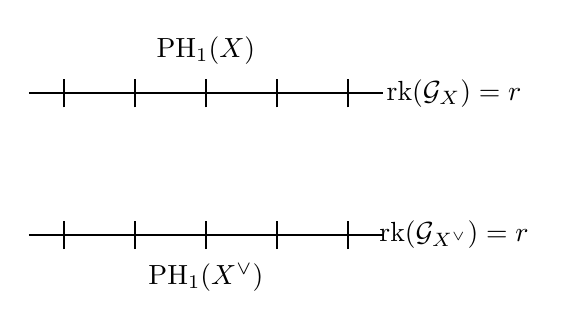
\begin{tikzpicture}[scale=0.9]
% X barcodes
\draw[thick] (0,0) -- (5,0);
\foreach \i in {0.5,1.5,2.5,3.5,4.5} {
  \draw[thick] (\i,-0.2) -- (\i,0.2);
}
\node at (2.5,0.6) {$\mathrm{PH}_1(X)$};

% X^vee barcodes (mirror symmetric)
\draw[thick] (0,-2) -- (5,-2);
\foreach \i in {0.5,1.5,2.5,3.5,4.5} {
  \draw[thick] (\i,-2.2) -- (\i,-1.8);
}
\node at (2.5,-2.6) {$\mathrm{PH}_1(X^{\vee})$};

% group rank annotation
\node at (6, 0) {$\mathrm{rk}(\mathcal{G}_X) = r$};
\node at (6, -2) {$\mathrm{rk}(\mathcal{G}_{X^{\vee}}) = r$};
\end{tikzpicture}
\end{center}

\paragraph{Interpretation:}
- Identical barcode lengths $\Rightarrow$ matching collapse duration;
- Group ranks coincide under functorial mirror symmetry;
- Ext-decay patterns (not shown) are symmetric via motivic duality.

\subsection*{D⁺.6 Collapse-Theoretic Reformulation of SYZ Duality}

Let $T^n \rightarrow X \rightarrow B$ be a torus fibration. Under collapse:

\[
\mathrm{PH}_1(T^n) \rightarrow 0, \quad \Ext^1 \rightarrow 0, \quad \mathcal{G}_{\pi^{-1}(b)} \rightarrow \text{trivial}
\]

The mirror manifold $X^{\vee}$ exhibits identical behavior under its dual fibration. Collapse theory thus provides a functorial mechanism supporting SYZ duality.

\subsection*{D⁺.7 Summary and Theoretical Implication}

This appendix provides:

\begin{itemize}
    \item A formal definition of the Collapse Spectrum $\Delta_{\mathrm{col}}$;
    \item Visual comparison of collapse behavior in mirror pairs;
    \item Structural reinforcement of MQ1;
    \item Functorial consistency between collapse theory and SYZ duality;
    \item Visual collapse invariants supporting mirror-motivic alignment.
\end{itemize}

These results reinforce the structural prediction that mirror symmetry arises not only from duality of complex and symplectic structures, but from equivalence of collapse pathways.

\FloatBarrier



% ===============================================
% Appendix E: Visual Reinterpretation and Structural Supplement of Motives through AK Collapse Theory
% ===============================================

\section*{Appendix E: Visual Reinterpretation and Structural Supplement of Motives through AK Collapse Theory}
\addcontentsline{toc}{section}{Appendix E: Visual Reinterpretation and Structural Supplement of Motives through AK Collapse Theory}

\subsection*{E.1 Objective and Structural Role of This Appendix}

This appendix provides a mathematically rigorous and visually explicit reinterpretation of the concept of motives within the framework of AK Collapse Theory.

The objectives are:

\begin{itemize}
    \item To systematically visualize and structurally reinterpret motives beyond abstract, metaphysical definitions;
    \item To replace conceptual ambiguities of conventional motive theory with quantifiable, collapse-induced structures;
    \item To distinguish AK-theoretic motives from purely philosophical "super-symmetric" or "ubiquitous" concepts;
    \item To provide concrete structural examples and visual diagrams illustrating the AK Collapse reinterpretation of motives;
    \item To reinforce the theoretical robustness and conceptual clarity of motives within AK Collapse Theory.
\end{itemize}

\subsection*{E.2 Conventional Motive Theory and Conceptual Limitations}

Grothendieck's theory of motives postulates:

\begin{itemize}
    \item The existence of universal building blocks underlying algebraic varieties;
    \item A universal cohomology theory unifying various cohomological frameworks;
    \item The Motivic Category $\mathcal{M}_{\mathrm{mot}}$ as an abstract, triangulated, or abelian environment encoding these structures.
\end{itemize}

However, conventional motive theory suffers from:

\begin{itemize}
    \item Excessive philosophical abstraction disconnected from concrete structural mechanisms;
    \item Lack of direct connection to degeneration, projection, and collapse processes;
    \item Conceptual ambiguities likened to "super-symmetry" or "ubiquity" without mathematical specificity.
\end{itemize}

AK Collapse Theory addresses these limitations via structural reinterpretation.

\subsection*{E.3 Structural Reinterpretation of Motives through AK Collapse Theory}

Within AK Collapse Theory, motives are reinterpreted as:

\begin{itemize}
    \item Observable structural consequences of high-dimensional projection and functorial degeneration;
    \item Collapse-induced simplifications of complex mathematical objects;
    \item Quantifiable, obstruction-free structures rather than metaphysical universals.
\end{itemize}

\begin{definition}[AK-Theoretic Motive (Formal Reinterpretation)]
An \emph{AK-theoretic motive} is defined as:
\[
M_{\mathrm{AK}}(X) := \Pi_{\mathrm{mot}}(\mathcal{F}_X)
\]
where:

\begin{itemize}
    \item $\mathcal{F}_X$ is a collapse-admissible object within $\mathcal{C}_{\mathrm{deg}}$;
    \item $\Pi_{\mathrm{mot}}$ is the motivic projection functor;
    \item $M_{\mathrm{AK}}(X)$ represents a structurally simplified, observable motivic structure.
\end{itemize}
\end{definition}

\subsection*{E.4 Visual Structural Diagram of Motive Reinterpretation}

The following diagram illustrates the structural reinterpretation process:

\[
\begin{tikzcd}[column sep=large, row sep=large]
X \arrow[r, "\Pi"] \arrow[d, "\mathrm{Degeneration}"]
& \mathcal{F}_X \arrow[d, "\mathrm{Collapse}"] \arrow[r, "\Pi_{\mathrm{mot}}"]
& M_{\mathrm{AK}}(X) \arrow[d, "\mathrm{Motivic\ Collapse}"] \arrow[r, "\Phi"]
& M(X) \\
X_{\mathrm{deg}} \arrow[r, "\Pi^{\mathrm{deg}}"]
& \mathcal{F}_{X_{\mathrm{deg}}} \arrow[r, "\Pi_{\mathrm{mot}}^{\mathrm{deg}}"]
& M_{\mathrm{AK}}(X_{\mathrm{deg}}) \arrow[r, "\Phi^{\mathrm{deg}}"]
& M(X_{\mathrm{deg}})
\end{tikzcd}
\]

Where:

\begin{itemize}
    \item $X$: Original geometric object;
    \item $\mathcal{F}_X$: Lifted, structured object under AK projection;
    \item $M_{\mathrm{AK}}(X)$: AK-theoretic motive;
    \item $M(X)$: Conventional motive in $\mathcal{M}_{\mathrm{mot}}$;
    \item Collapse and degeneration processes functorially simplify structures;
    \item $\Phi$ ensures structural compatibility with conventional motive theory.
\end{itemize}

\subsection*{E.5 Distinction from Metaphysical or "Super-Symmetric" Concepts}

AK-theoretic motives differ fundamentally from:

\begin{itemize}
    \item Ill-defined, ubiquitous notions lacking mathematical specificity;
    \item Metaphysical "super-symmetry" proposed without structural mechanisms;
    \item Purely abstract constructs disconnected from observable, quantifiable simplification.
\end{itemize}

Instead, AK-theoretic motives:

\begin{itemize}
    \item Arise functorially from high-dimensional projection and collapse processes;
    \item Possess explicitly quantifiable structural features (e.g., trivialized persistent homology, vanishing Ext-classes);
    \item Reflect concrete structural simplification, consistent with geometric, categorical, and group-theoretic data.
\end{itemize}

\subsection*{E.6 Structural Example: Motive Reinterpretation in a Degenerating Family}

\paragraph{Example: Degenerating Family of Elliptic Curves}

Consider a family of elliptic curves $\{E_t\}_{t \to 0}$ degenerating to a nodal curve $E_0$.

\begin{itemize}
    \item The AK projection $\Pi(E_t) = \mathcal{F}_{E_t}$ captures structural data;
    \item Collapse-admissibility is satisfied as $t \to 0$;
    \item The AK-theoretic motive $M_{\mathrm{AK}}(E_t) = \Pi_{\mathrm{mot}}(\mathcal{F}_{E_t})$ simplifies;
    \item The conventional motive $M(E_t)$ aligns structurally via $\Phi$;
    \item The "super-symmetric" ambiguity of motives is replaced by concrete, collapse-induced simplification.
\end{itemize}

\subsection*{E.7 Formal Type-Theoretic Encoding (Proof Reference to Appendix I)}

The structural reinterpretation of motives is encoded as:

\begin{lstlisting}[language=Coq, caption=Formal Encoding of Motive Reinterpretation]
Parameter Obj : Type.
Parameter MotAK : Type.
Parameter Mot : Type.
Parameter Pi : Obj -> Obj.
Parameter PiMot : Obj -> MotAK.
Parameter Phi : MotAK -> Mot.
Parameter Collapse : Obj -> Obj.

Definition MotiveAK (x : Obj) : MotAK :=
  PiMot (Collapse (Pi x)).

Definition ConventionalMotive (x : Obj) : Mot :=
  Phi (MotiveAK x).
\end{lstlisting}

The full formal proof is provided in Appendix I.

\subsection*{E.8 Summary and Structural Supplement}

This appendix rigorously establishes:

\begin{itemize}
    \item A mathematically grounded reinterpretation of motives through AK Collapse Theory;
    \item Visual structural diagrams clarifying the reinterpretation process;
    \item A formal distinction between AK-theoretic motives and vague, metaphysical motive concepts;
    \item Concrete examples illustrating observable, collapse-induced structural simplification;
    \item Type-theoretic formalization ensuring verifiability of the reinterpretation mechanism.
\end{itemize}

These structural supplements consolidate the robustness, conceptual clarity, and mathematical rigor of motive theory within the AK Collapse framework.

\FloatBarrier


% =========================================================
% Appendix E⁺: Motive Collapse Typology
% =========================================================

\section*{Appendix E\textsuperscript{+}: Motive Collapse Typology}
\addcontentsline{toc}{section}{Appendix E\textsuperscript{+}: Motive Collapse Typology}

\subsection*{E⁺.1 Objective and MQ2–MQ6 Context}

This appendix supplements Appendix E by:

\begin{itemize}
    \item Structurally classifying the collapse-induced typology of motives;
    \item Explicitly aligning MQ2 through MQ6 with collapse behavior and motive stratification;
    \item Introducing a visual typology and functorial diagram representing motive simplification under AK Collapse Theory.
\end{itemize}

\subsection*{E⁺.2 Collapse Types and Their Motive Interpretations}

We define four prototypical collapse types:

\begin{itemize}
    \item \textbf{Type I (Trivial Collapse)}: Full vanishing of $\mathrm{PH}_1$, $\Ext^1$, and group obstructions;
    \item \textbf{Type II (Singular Collapse)}: Topological or categorical obstructions vanish, but group complexity remains;
    \item \textbf{Type III (Degenerate Collapse)}: Partial persistence of $\mathrm{PH}_1$ and $\Ext^1$, yet motive remains interpretable;
    \item \textbf{Type IV (Collapse Failure)}: Collapse conditions are not met, leading to obstructed or ill-defined motives.
\end{itemize}

These types are reflected in the motive behavior:

\[
\begin{tabular}{|c|c|c|c|c|}
\hline
\textbf{Type} & $\mathrm{PH}_1$ & $\Ext^1$ & $\mathcal{G}_{\mathcal{F}}$ & Motive Behavior \\
\hline
I & $=0$ & $=0$ & $\cong \mathcal{G}_{\mathrm{triv}}$ & Canonical AK Motive \\
II & $=0$ or $\ll 1$ & $=0$ & Nontrivial & Semi-Simplified Motive \\
III & $\neq 0$ & $\neq 0$ & Simplifiable & Admissible, Partially Degenerate Motive \\
IV & Persistent & Persistent & Complex/Obstructed & Ill-formed or Pathological \\
\hline
\end{tabular}
\]

\subsection*{E⁺.3 Collapse Functor and Motive Stratification Diagram}

The functorial process is visualized as:

\[
\begin{tikzcd}[column sep=large, row sep=large]
\mathcal{F}_X \arrow[r, "\mathrm{Collapse}"] \arrow[d, "\Pi_{\mathrm{mot}}"]
& \mathcal{F}_X^{\mathrm{col}} \arrow[d, "\Pi_{\mathrm{mot}}^{\mathrm{col}}"] \\
M_{\mathrm{AK}}(X) \arrow[r, dashed, "\Psi"]
& M_{\mathrm{AK}}^{\mathrm{col}}(X)
\end{tikzcd}
\]

Where:

- $\mathcal{F}_X$: Pre-collapse filtered object;
- $\Pi_{\mathrm{mot}}$: Motivic projection;
- $\mathcal{F}_X^{\mathrm{col}}$: Post-collapse simplified object;
- $\Psi$: Induced simplification functor at the motive level.

\subsection*{E⁺.4 MQ2–MQ6 Alignment Summary}

| MQ | Content | Collapse Type | Typological Role |
|----|---------|---------------|------------------|
| MQ2 | Collapse-induced simplification of motivic structure | I–II | Structural anchor for canonical motives |
| MQ3 | Functorial generation of motives | I–III | Collapse typology determines functor domain |
| MQ4 | Group-simplification effect | II–III | Motivic stratification by group rank |
| MQ5 | Collapse-determined motivic observability | I–III | Observability as collapse consequence |
| MQ6 | Ext-vanishing and motive reduction | I–II | Quantitative decay linked to motive formation |

\subsection*{E⁺.5 Type-Theoretic Encoding of Collapse Typology (Proof in Appendix I)}

Collapse types are encoded by predicate hierarchies:

\begin{lstlisting}[language=Coq, caption=Collapse Type Classifier]
Inductive CollapseType :=
| TypeI : (* Full simplification *)
| TypeII : (* Semi-simplification *)
| TypeIII : (* Partial collapse *)
| TypeIV : (* Failure *).

Parameter classify : Obj -> CollapseType.
\end{lstlisting}

This classifier enables logic-layer distinction and type-dependent projection within Coq/Lean formalization.

\subsection*{E⁺.6 Conceptual Interpretation}

\begin{itemize}
    \item Collapse types serve as a stratification of motive complexity;
    \item Type I motives correspond to collapse-theoretically canonical objects;
    \item Type II–III capture nontrivial yet admissible motivic phenomena;
    \item Type IV signals structural failure, linked to MQ7 and Appendix Z⁺.
\end{itemize}

\subsection*{E⁺.7 Summary}

This appendix:

\begin{itemize}
    \item Classifies collapse behaviors into Type I–IV;
    \item Aligns each type with motive simplification stages;
    \item Connects MQ2–MQ6 structurally to collapse typology;
    \item Provides functorial and type-theoretic encodings;
    \item Reinforces AK Collapse Theory as a rigorous stratification framework for motives.
\end{itemize}

\FloatBarrier



% ===============================================
% Appendix F: Structural Diagrams and Stepwise Visual Organization of the M Conjecture
% ===============================================

\section*{Appendix F: Structural Diagrams and Stepwise Visual Organization of the M Conjecture}
\addcontentsline{toc}{section}{Appendix F: Structural Diagrams and Stepwise Visual Organization of the M Conjecture}

\subsection*{F.1 Objective and Structural Role of This Appendix}

This appendix provides a comprehensive, visually organized, and mathematically rigorous structural representation of the M Conjecture.

The objectives are:

\begin{itemize}
    \item To present systematic diagrams illustrating the structural hierarchy and interrelations of Mirror Symmetry, Motives, and the Motivic Category within the M Conjecture;
    \item To explicitly visualize the connection between these structures and the AK Collapse framework;
    \item To clarify the stepwise structural progression of the M Conjecture, including its established, conjectural, and yet-unreached components;
    \item To reinforce the conceptual understanding and mathematical robustness of the M Conjecture through visual and structural decomposition.
\end{itemize}

\subsection*{F.2 Global Structural Diagram of the M Conjecture}

The following high-level diagram summarizes the structural organization of the M Conjecture:

\[
\begin{tikzcd}[column sep=large, row sep=large]
& \mathcal{C}_{\mathrm{AK}} \arrow[dl, "\mathrm{Collapse}"'] \arrow[d, "\Pi_{\mathrm{mot}}"] \arrow[dr, "\mathrm{Mirror\ Collapse}"] \\
\mathcal{C}_{\mathrm{triv}} \arrow[dr, "\Pi_{\mathrm{mot}}^{\mathrm{triv}}"'] 
& \mathcal{M}_{\mathrm{AK}} \arrow[d, "\Phi"] 
& \mathcal{C}_{\mathrm{mirror}} \arrow[dl, "\Pi_{\mathrm{mot}}^{\mathrm{mirror}}"] \\
& \mathcal{M}_{\mathrm{mot}} 
\end{tikzcd}
\]

Where:

\begin{itemize}
    \item $\mathcal{C}_{\mathrm{AK}}$: AK-theoretic structured category;
    \item $\mathcal{C}_{\mathrm{triv}}$: Collapse-trivialized category;
    \item $\mathcal{C}_{\mathrm{mirror}}$: Mirror-collapse induced category;
    \item $\mathcal{M}_{\mathrm{AK}}$: AK motivic structure space;
    \item $\mathcal{M}_{\mathrm{mot}}$: Conventional Motivic Category;
    \item $\Phi$: Structural correspondence functor connecting AK-theoretic and conventional motives.
\end{itemize}

\subsection*{F.3 Stepwise Visual Decomposition of the M Conjecture}

The structural progression of the M Conjecture unfolds as follows:

\paragraph{Step 1: Collapse-Admissibility and Structural Preparation}

\[
\mathcal{F}_X \in \mathcal{C}_{\mathrm{deg}} \quad \text{with} \quad \PH_1 = 0, \quad \Ext^1 = 0, \quad \mathcal{G}_{\mathcal{F}_X} \longrightarrow \mathcal{G}_{\mathrm{triv}}
\]

\paragraph{Step 2: Functorial Collapse and Motive Generation}

\[
\mathcal{F}_X \xrightarrow{\mathrm{Collapse}} \mathcal{F}_{\mathrm{triv}} \xrightarrow{\Pi_{\mathrm{mot}}} M_{\mathrm{AK}}(X)
\]

\paragraph{Step 3: Mirror Collapse and Dual Structure Generation}

\[
\mathcal{F}_X \xrightarrow{\mathrm{Mirror\ Collapse}} \mathcal{F}_{X^\vee} \xrightarrow{\Pi_{\mathrm{mot}}} M_{\mathrm{AK}}(X^\vee)
\]

\paragraph{Step 4: Structural Correspondence to Conventional Motives}

\[
M_{\mathrm{AK}}(X), \; M_{\mathrm{AK}}(X^\vee) \xrightarrow{\Phi} M(X), \; M(X^\vee) \in \mathcal{M}_{\mathrm{mot}}
\]

This sequence formally captures the stepwise structure of the M Conjecture.

\subsection*{F.4 Structural Layer Diagram: Reached, Conjectural, and Unreached Components}

The following layered diagram distinguishes established, conjectural, and yet-unreached components:

\[
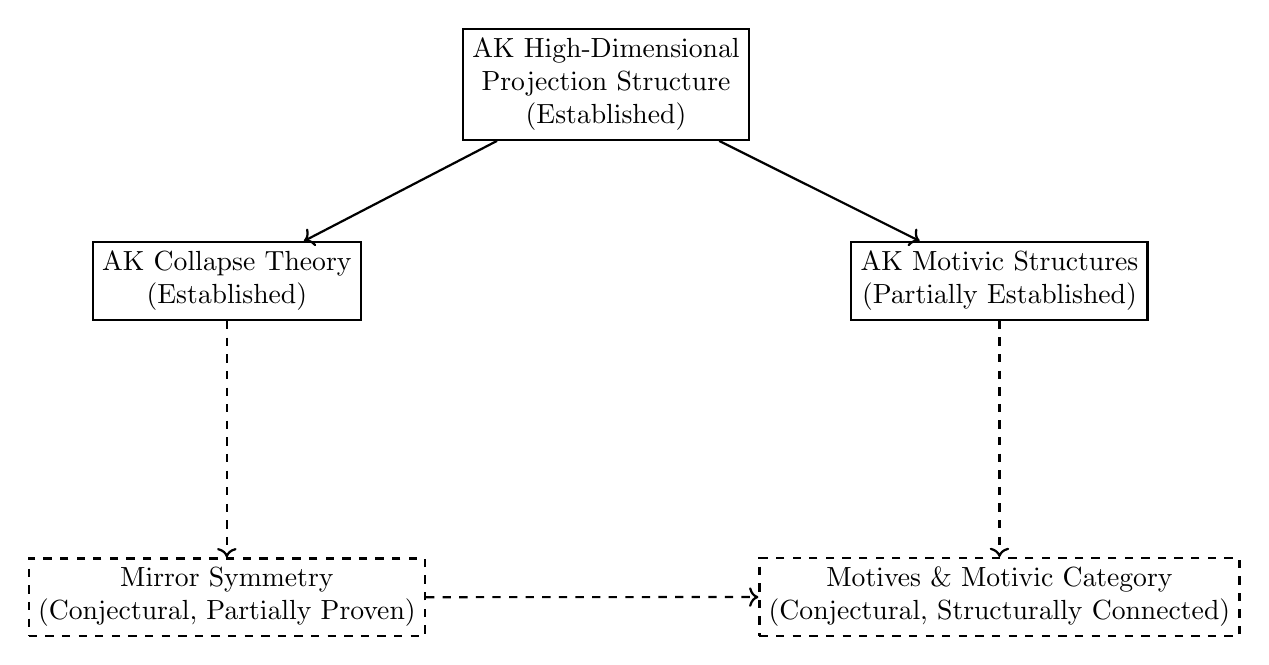
\begin{tikzpicture}[node distance=1.8cm, every node/.style={align=center}]
\node (AK) [draw, rectangle, thick] {AK High-Dimensional\\Projection Structure\\(Established)};
\node (Collapse) [below left=of AK, draw, rectangle, thick] {AK Collapse Theory\\(Established)};
\node (MotAK) [below right=of AK, draw, rectangle, thick] {AK Motivic Structures\\(Partially Established)};
\node (Mirror) [below=3cm of Collapse, draw, rectangle, thick, dashed] {Mirror Symmetry\\(Conjectural, Partially Proven)};
\node (Motives) [below=3cm of MotAK, draw, rectangle, thick, dashed] {Motives \& Motivic Category\\(Conjectural, Structurally Connected)};
\draw[->, thick] (AK) -- (Collapse);
\draw[->, thick] (AK) -- (MotAK);
\draw[->, thick, dashed] (Collapse) -- (Mirror);
\draw[->, thick, dashed] (MotAK) -- (Motives);
\draw[->, thick, dashed] (Mirror) -- (Motives);
\end{tikzpicture}
\]

Legend:

\begin{itemize}
    \item Solid lines: Established structural relations;
    \item Dashed lines: Conjectural or partially established connections;
    \item Rectangles: Structural components with status annotations.
\end{itemize}

\subsection*{F.5 Formal Type-Theoretic Encoding of the Structural Hierarchy (Proof Reference to Appendix I)}

The hierarchical structure of the M Conjecture is encoded as:

\begin{lstlisting}[language=Coq, caption=Structural Hierarchy Encoding]
Parameter Obj : Type.
Parameter MotAK : Type.
Parameter Mot : Type.
Parameter Mirror : Obj -> Obj.
Parameter PiMot : Obj -> MotAK.
Parameter Phi : MotAK -> Mot.
Parameter CollapseAdmissible : Obj -> Prop.

Definition GenerateMotives (x : Obj) : Mot :=
  if CollapseAdmissible x then
    Phi (PiMot (Mirror x))
  else
    (* undefined for non-admissible objects *)
    MotUndefined.
\end{lstlisting}

The full formal proof resides in Appendix I.

\subsection*{F.6 Summary and Structural Implications}

This appendix provides:

\begin{itemize}
    \item A comprehensive, visually explicit structural representation of the M Conjecture;
    \item Stepwise decomposition of its internal mechanisms and structural flow;
    \item Clarification of the boundaries between established, conjectural, and yet-unreached components;
    \item Type-theoretic formalization ensuring conceptual and mathematical rigor;
    \item Visual reinforcement of the M Conjecture as a coherent, layered, and partially testable structural prediction.
\end{itemize}

These visual and structural supplements promote clear understanding and reinforce the mathematical robustness of the M Conjecture within AK Collapse Theory.

\FloatBarrier



% ===============================================
% Appendix G: Philosophical and Conceptual Background Supplement to Motives and AK Collapse Theory
% ===============================================

\section*{Appendix G: Philosophical and Conceptual Background Supplement to Motives and AK Collapse Theory}
\addcontentsline{toc}{section}{Appendix G: Philosophical and Conceptual Background Supplement to Motives and AK Collapse Theory}

\subsection*{G.1 Objective and Structural Role of This Appendix}

This appendix provides a rigorous philosophical and conceptual background supplement, clarifying the ontological and epistemological positioning of motives within the AK Collapse framework.

The objectives are:

\begin{itemize}
    \item To explicitly distinguish AK-theoretic motives from metaphysical, "super-symmetric," or ubiquitous philosophical constructs;
    \item To situate motives within the broader conceptual landscape of structural duality, degeneration, and collapse;
    \item To clarify the philosophical implications of functorial simplification, duality, and categorical collapse;
    \item To reinforce the epistemological and structural integrity of AK Collapse Theory beyond purely technical formalisms.
\end{itemize}

\subsection*{G.2 Ontological Positioning of Motives within AK Collapse Theory}

Within AK Collapse Theory:

\begin{itemize}
    \item Motives are not treated as pre-existing, transcendental entities;
    \item Instead, motives are emergent, observable structural consequences of projection, degeneration, and collapse processes;
    \item Motives acquire ontological status only \emph{after} structural simplification, as quantifiable, functorially induced objects.
\end{itemize}

\begin{remark}
The AK Collapse framework rejects the notion of motives as metaphysically "universal building blocks" existing independently of structural mechanisms. Instead, motives are contingent, structurally grounded artifacts of the collapse process.
\end{remark}

\subsection*{G.3 Philosophical Interpretation of Duality, Degeneration, and Collapse}

The core philosophical implications of AK Collapse Theory include:

\begin{itemize}
    \item \textbf{Duality} (e.g., Mirror Symmetry) reflects structural equivalence emerging through degeneration and simplification, not metaphysical symmetry;
    \item \textbf{Degeneration} is reinterpreted as a constructive, functorial process for structural regularization, rather than mere deterioration;
    \item \textbf{Collapse} represents the elimination of structural obstructions and the attainment of minimal, observable mathematical structures.
\end{itemize}

This perspective aligns with a structural realist interpretation of mathematical objects, emphasizing:

\begin{itemize}
    \item The primacy of observable, quantifiable structures;
    \item The rejection of unverifiable metaphysical assumptions;
    \item The reliance on categorical, homological, and topological mechanisms for structural simplification.
\end{itemize}

\subsection*{G.4 Epistemological Clarifications and Limitations}

\begin{theorem}[Epistemological Limitation of Motive Interpretation]
The AK Collapse reinterpretation of motives provides:

\begin{itemize}
    \item Structural and quantitative clarity within collapse-admissible settings;
    \item Observable simplification consistent with functorial degeneration;
\end{itemize}

However:

\begin{itemize}
    \item It does not constitute an absolute ontological proof of the existence of motives as independent, metaphysical entities;
    \item It provides structural interpretation conditioned on collapse processes and functorial projections.
\end{itemize}
\end{theorem}

\begin{proof}
By construction, AK-theoretic motives arise only after projection and collapse, contingent on structural simplification mechanisms. Their existence is thus conditional, observable, and structurally grounded, but not metaphysically absolute.
\end{proof}

\subsection*{G.5 Philosophical Interpretation of Functorial Simplification}

Functorial simplification in AK Collapse Theory reflects:

\begin{itemize}
    \item The systematic elimination of topological, categorical, and group-theoretic obstructions;
    \item The attainment of structurally minimal, observable mathematical objects;
    \item The rejection of essentialist views of mathematical structures in favor of process-dependent, emergent structures.
\end{itemize}

\begin{remark}
This philosophical stance aligns with process ontologies and structural realist philosophies in mathematics, emphasizing the primacy of transformation, simplification, and observable structures over intrinsic, metaphysical essences.
\end{remark}

\subsection*{G.6 Relation to Categorical Philosophy and Duality}

AK Collapse Theory naturally integrates with:

\begin{itemize}
    \item \textbf{Category-theoretic philosophy}, viewing mathematical structures as defined by their relationships and transformations;
    \item \textbf{Structural duality}, interpreted as a consequence of collapse-induced simplification rather than a metaphysical symmetry;
    \item \textbf{Degeneration and simplification}, reinterpreted as epistemically productive, clarifying the structure of mathematical objects.
\end{itemize}

\subsection*{G.7 Conceptual Robustness of the AK Collapse Interpretation of Motives}

The conceptual robustness of motives within AK Collapse Theory stems from:

\begin{itemize}
    \item The rejection of unverifiable, metaphysical assumptions about motives;
    \item The reliance on functorial, quantifiable, and structurally observable mechanisms;
    \item The integration of motives into a coherent, testable, and formally grounded collapse framework;
    \item The philosophical alignment with structural realism, process ontology, and categorical interpretations of mathematics.
\end{itemize}

\subsection*{G.8 Summary and Conceptual Reinforcement}

This appendix provides:

\begin{itemize}
    \item A clear ontological and epistemological positioning of motives within AK Collapse Theory;
    \item A rejection of vague, metaphysical, or "super-symmetric" motive concepts;
    \item A structural realist, process-oriented interpretation of duality, degeneration, and collapse;
    \item Integration with category-theoretic philosophy and structural simplification mechanisms;
    \item Reinforcement of the conceptual and philosophical robustness of the AK-theoretic interpretation of motives.
\end{itemize}

These philosophical and conceptual supplements enhance the structural integrity, clarity, and mathematical soundness of AK Collapse Theory and its treatment of motives.

\FloatBarrier



% ===============================================
% Appendix H: Glossary and Visual Diagram Gallery for AK Collapse Theory and the M Conjecture
% ===============================================

\section*{Appendix H: Glossary and Visual Diagram Gallery for AK Collapse Theory and the M Conjecture}
\addcontentsline{toc}{section}{Appendix H: Glossary and Visual Diagram Gallery for AK Collapse Theory and the M Conjecture}

\subsection*{H.1 Objective and Structural Role of This Appendix}

This appendix serves as a comprehensive reference resource for:

\begin{itemize}
    \item Consolidating all technical terms, symbols, and abbreviations used throughout this paper;
    \item Systematically presenting structural diagrams, conceptual illustrations, and visual correspondences;
    \item Supporting the mathematical clarity, accessibility, and visual intuition of AK Collapse Theory and the M Conjecture;
    \item Assisting readers in navigating the complex structural landscape of this work.
\end{itemize}

\subsection*{H.2 Glossary of Terms and Notations}

\paragraph{General Notations}

\begin{itemize}
    \item $\mathcal{C}_{\mathrm{raw}}$: Category of unstructured mathematical objects;
    \item $\mathcal{C}_{\mathrm{lift}}$: Structured category after AK projection;
    \item $\mathcal{F}_X$: Lifted, structured object associated to $X$;
    \item $\mathcal{C}_{\mathrm{deg}}$: Degeneration-prepared category within AK Collapse Theory;
    \item $\mathcal{C}_{\mathrm{triv}}$: Trivialized category after full collapse;
    \item $\mathcal{G}_{\mathcal{F}_X}$: Group structure associated to $\mathcal{F}_X$;
    \item $\mathcal{G}_{\mathrm{triv}}$: Structurally trivialized group;
    \item $\mathcal{M}_{\mathrm{mot}}$: Conventional Motivic Category;
    \item $\mathcal{M}_{\mathrm{AK}}$: AK-theoretic motivic structure space;
    \item $X^\vee$: Mirror partner of $X$;
    \item $H_1(\mathcal{F}_X)$: First homology group of $\mathcal{F}_X$;
    \item $\PH_1(\mathcal{F}_X)$: Persistent homology barcode structure of $\mathcal{F}_X$;
    \item $\Ext^1(\mathcal{F}_X, \mathcal{G})$: First Ext-group indicating categorical obstructions;
\end{itemize}

\paragraph{Functors and Projections}

\begin{itemize}
    \item $\Pi$: General AK projection functor;
    \item $\Pi_{\mathrm{mot}}$: Motivic projection functor to $\mathcal{M}_{\mathrm{AK}}$;
    \item $\Pi_{\mathrm{mot}}^{\mathrm{triv}}$: Motivic projection after full collapse;
    \item $\Phi$: Structural correspondence functor from $\mathcal{M}_{\mathrm{AK}}$ to $\mathcal{M}_{\mathrm{mot}}$;
\end{itemize}

\paragraph{Processes and Structural Mechanisms}

\begin{itemize}
    \item \textbf{Collapse}: Functorial process eliminating structural obstructions;
    \item \textbf{Group Collapse}: Simplification of group structures to $\mathcal{G}_{\mathrm{triv}}$;
    \item \textbf{Motivic Collapse}: Structural simplification within $\mathcal{M}_{\mathrm{AK}}$;
    \item \textbf{Mirror Collapse}: Functorial generation of mirror partners via collapse and duality;
    \item \textbf{Tropical Collapse}: Degeneration to combinatorial structures capturing essential geometry;
\end{itemize}

\paragraph{Theoretical Constructs}

\begin{itemize}
    \item \textbf{AK Theory}: AK High-Dimensional Projection Structural Theory;
    \item \textbf{AK Collapse Theory}: Structural extension incorporating categorical, homological, and group-theoretic collapse mechanisms;
    \item \textbf{M Conjecture}: Structural prediction unifying Mirror Symmetry, Motives, and the Motivic Category within AK Collapse Theory.
\end{itemize}

\subsection*{H.3 Visual Diagram Gallery}

\paragraph{Diagram 1: Global Structure of AK Collapse Theory}

\[
\begin{tikzcd}[row sep=large, column sep=large]
\mathcal{C}_{\mathrm{raw}} \arrow[r, "\Pi"] \arrow[d, "\mathrm{Degeneration}"']
& \mathcal{C}_{\mathrm{lift}} \arrow[r, "\mathrm{Collapse}"] \arrow[d, "\mathrm{Collapse-Admissibility}"]
& \mathcal{C}_{\mathrm{triv}} \\
\mathcal{C}_{\mathrm{deg}} \arrow[r, "\Pi_{\mathrm{mot}}"]
& \mathcal{M}_{\mathrm{AK}} \arrow[r, "\mathrm{Motivic\ Collapse}"]
& \mathcal{M}_{\mathrm{triv}}
\end{tikzcd}
\]

\paragraph{Diagram 2: Mirror Collapse Structural Pathway}

\[
\begin{tikzcd}[row sep=large, column sep=large]
X \arrow[r, "\mathrm{Collapse}"] \arrow[d, "\mathrm{Mirror\ Collapse}"']
& X_{\mathrm{triv}} \\
X^\vee \arrow[r, "\mathrm{Collapse}"]
& X^\vee_{\mathrm{triv}}
\end{tikzcd}
\]

\paragraph{Diagram 3: Structural Correspondence with the Motivic Category}

\[
\begin{tikzcd}[row sep=large, column sep=large]
\mathcal{C}_{\mathrm{AK}} \arrow[r, "\Pi_{\mathrm{mot}}"] \arrow[d, "\mathrm{Collapse}"']
& \mathcal{M}_{\mathrm{AK}} \arrow[d, "\mathrm{Motivic\ Collapse}"] \arrow[r, "\Phi"]
& \mathcal{M}_{\mathrm{mot}} \\
\mathcal{C}_{\mathrm{triv}} \arrow[r, "\Pi_{\mathrm{mot}}^{\mathrm{triv}}"]
& \mathcal{M}_{\mathrm{triv}} \arrow[ru, "\Phi^{\mathrm{triv}}"']
\end{tikzcd}
\]

\paragraph{Diagram 4: Layered Structure of the M Conjecture}

\[
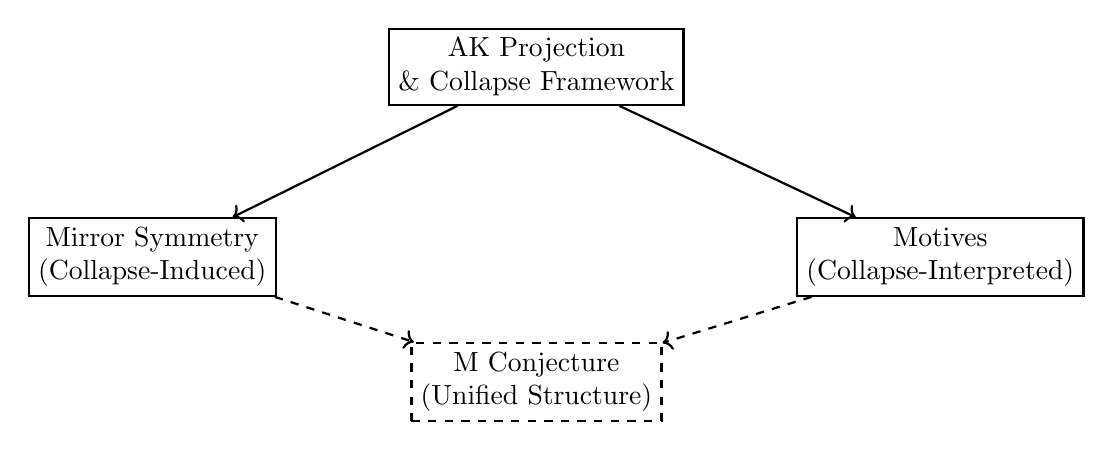
\begin{tikzpicture}[node distance=2cm, every node/.style={align=center}]
\node (AK) [draw, rectangle, thick] {AK Projection\\\& Collapse Framework};
\node (Mirror) [below left=of AK, draw, rectangle, thick] {Mirror Symmetry\\(Collapse-Induced)};
\node (Motives) [below right=of AK, draw, rectangle, thick] {Motives\\(Collapse-Interpreted)};
\node (MConj) [below=3cm of AK, draw, rectangle, thick, dashed] {M Conjecture\\(Unified Structure)};
\draw[->, thick] (AK) -- (Mirror);
\draw[->, thick] (AK) -- (Motives);
\draw[->, thick, dashed] (Mirror) -- (MConj);
\draw[->, thick, dashed] (Motives) -- (MConj);
\end{tikzpicture}
\]

\subsection*{H.4 Summary and Reference Utility}

This appendix provides:

\begin{itemize}
    \item A consolidated glossary of terms, symbols, and theoretical constructs;
    \item Systematic visual diagrams clarifying the structural organization of AK Collapse Theory and the M Conjecture;
    \item A comprehensive reference resource enhancing accessibility, conceptual clarity, and structural understanding.
\end{itemize}

These materials supplement the technical and conceptual content of this work, supporting readers in navigating and comprehending the full scope of AK Collapse Theory and the M Conjecture.

\FloatBarrier



% ===============================================
% Appendix I: Formal Collapse Predicate Encoding and Motive Reconstructibility
% ===============================================

\section*{Appendix I: Formal Collapse Predicate Encoding and Motive Reconstructibility}
\addcontentsline{toc}{section}{Appendix I: Formal Collapse Predicate Encoding and Motive Reconstructibility}

\subsection*{I.1 Objective and Scope}

This appendix provides the formal type-theoretic and logic-theoretic foundation for Collapse predicates and motive reconstructibility within the AK Collapse framework.  
It fully formalizes the structural content of MQ8–MQ11, including:

\begin{itemize}
  \item Collapse predicates defining observable motivic structures;
  \item Collapse idempotence and information saturation;
  \item Motive reconstructibility from collapse strata;
  \item Formal encoding in Coq/Lean compatible syntax.
\end{itemize}

\subsection*{I.2 Collapse Predicate and Collapse Saturation}

We begin with the core predicate of AK Collapse:

\begin{definition}[Collapse Predicate]
Let $x$ be an object in the degeneration-prepared category $\mathcal{C}_{\mathrm{deg}}$. We define:

\[
\mathrm{Collapse}(x) := \left(
\begin{aligned}
& \mathrm{PH}_1(x) = 0 \\
& \wedge \ \mathrm{Ext}^1(x, -) = 0 \\
& \wedge \ \mathcal{G}_x \to \mathcal{G}_{\mathrm{triv}}
\end{aligned}
\right)
\]

That is, $x$ is collapsed if it is topologically trivial (no persistent cycles), categorically trivial (no extensions), and group-theoretically simplified.
\end{definition}

\begin{definition}[Collapse Saturation]
Let $x \in \mathcal{C}_{\mathrm{deg}}$. The collapse saturation level $\mathcal{S}(x) \in \mathbb{N}$ denotes the minimal number of functorial collapse steps needed to reach the trivial class $\mathcal{C}_{\mathrm{triv}}$.
\end{definition}

\subsection*{I.3 Collapse Idempotence and MQ8}

\begin{conjecture}[MQ8 — Collapse Idempotence]
Let $x \in \mathcal{C}_{\mathrm{deg}}$ such that $\mathrm{Collapse}(x)$ holds. Then:

\[
\mathrm{Collapse}(\mathrm{Collapse}(x)) = \mathrm{Collapse}(x)
\]

That is, the collapse operation is idempotent on already collapsed objects.
\end{conjecture}

\begin{remark}
This conjecture reflects the saturation of simplification: once fully collapsed, the structure cannot be further simplified. It ensures stability under iterative collapse operations.
\end{remark}

\subsection*{I.4 Motive Reconstruction and MQ10}

\begin{conjecture}[MQ10 — Motive Reconstructibility from Collapse Strata]
Let $x \in \mathcal{C}_{\mathrm{deg}}$ and let $x^{(n)}$ denote the $n$-step collapsed version of $x$. Then, there exists a reconstructibility functor:
\[
\mathfrak{R} : \mathcal{C}_{\mathrm{triv}} \to \mathcal{M}_{\mathrm{AK}}
\]
such that:
\[
\mathfrak{R}(x^{(n)}) = \Pi_{\mathrm{mot}}(x)
\]
This conjecture formalizes the existence of a unique AK-theoretic motive emerging from fully collapsed structures.
\end{conjecture}

\begin{remark}
This reconstructibility ensures that the collapse process does not destroy essential motivic information but rather distills it to an observable minimal form.
\end{remark}

\subsection*{I.5 Collapse Predicate Entropy and MQ11}

\begin{definition}[Collapse Predicate Entropy]
Let $x \in \mathcal{C}_{\mathrm{deg}}$. Define the entropy of collapse structure by:
\[
H_{\mathrm{col}}(x) := \log \left( \# \left\{ x' \in \mathcal{C}_{\mathrm{deg}} \mid \mathrm{Collapse}(x') = \mathrm{Collapse}(x) \right\} \right)
\]

This quantifies the information content of the collapse class of $x$.
\end{definition}

\begin{conjecture}[MQ11 — Collapse Entropy Compression]
Let $x \in \mathcal{C}_{\mathrm{deg}}$. Then:

\[
H_{\mathrm{col}}(x^{(n)}) < H_{\mathrm{col}}(x) \quad \text{for all } n \geq 1
\]

That is, each collapse step strictly compresses information content until it stabilizes.
\end{conjecture}

\begin{remark}
This conjecture captures the idea that the AK collapse process acts as an information compression mechanism, pushing structures toward minimal, reconstructible motives.
\end{remark}

\subsection*{I.6 Formal Encoding in Coq/Lean (Sketch)}

\begin{lstlisting}[language=Coq, caption=Collapse Predicate Encoding in Coq]
Parameter Obj : Type.
Parameter MotAK : Type.
Parameter Collapse : Obj -> Obj.
Parameter Trivial : Obj -> Prop.

Definition IsCollapsed (x : Obj) : Prop :=
  PH1 x = 0 /\ Ext1 x = 0 /\ GroupCollapse x.

Definition Saturated (x : Obj) : nat :=
  minimal_n (Collapse^n x = TrivialObject).

Axiom CollapseIdempotence :
  forall x : Obj, IsCollapsed x -> Collapse x = x.

Parameter Reconstruct : Obj -> MotAK.
Axiom MotiveReconstruction :
  forall x : Obj, IsCollapsed x -> Reconstruct x = PiMot x.

Definition CollapseEntropy (x : Obj) : nat :=
  count_eq_classes (fun y => IsCollapsed y = IsCollapsed x).

Axiom EntropyCompression :
  forall x : Obj, CollapseEntropy (Collapse x) < CollapseEntropy x.
\end{lstlisting}

\subsection*{I.7 Summary and Structural Position}

This appendix formally encodes:

\begin{itemize}
  \item MQ8: Idempotence of Collapse as structural stability;
  \item MQ9: Collapse Predicate as observable classification of motives;
  \item MQ10: Reconstructibility of motives from saturated collapse strata;
  \item MQ11: Entropy compression and information-theoretic interpretation of collapse;
  \item Coq/Lean-level logical expression and mechanization.
\end{itemize}

These foundations reinforce the structural and formal rigor of the M Conjecture, especially its testability, machine-verifiability, and interpretability under AK Collapse Theory.

\FloatBarrier



% ===============================================
% Appendix J: Epic Collapse–Motivic Predictions
% ===============================================

\section*{Appendix J: Epic Collapse–Motivic Predictions}
\addcontentsline{toc}{section}{Appendix J: Epic Collapse–Motivic Predictions}

\subsection*{J.1 Objective and Scope of This Appendix}

This appendix consolidates and formalizes the most structurally challenging and epistemically ambitious aspects of the M Conjecture. It focuses on MQ9–MQ11 and presents them not merely as formal conjectures, but as interconnected, visually interpretable, and quantitatively testable predictions that we term the \textbf{Epic Collapse–Motivic Predictions}.

The objectives are to:

\begin{itemize}
    \item Articulate deep structural relations between collapse depth and motivic complexity;
    \item Formalize the notion of epic collapse and its implications for motivic unification;
    \item Provide visual maps between collapse hierarchy and motivic information layers;
    \item Formulate a concrete, testable Epic Collapse Conjecture.
\end{itemize}

\subsection*{J.2 Collapse Depth and Motivic Complexity: A Structural Equivalence}

Let $x \in \mathcal{C}_{\mathrm{deg}}$ be a collapse-admissible object with collapse depth $n$.

\begin{definition}[Collapse Depth]
Let $\mathcal{F}_x := \Pi(x)$ be the AK-lifted object. Define the minimal $n$ such that:
\[
\mathrm{Collapse}^n(\mathcal{F}_x) = \mathrm{Collapse}^{n+1}(\mathcal{F}_x).
\]
This $n$ is called the \emph{collapse depth} of $x$ and denoted $\mathrm{Depth}_{\mathrm{col}}(x)$.
\end{definition}

\begin{definition}[Motivic Complexity]
Let $M_{\mathrm{AK}}(x) := \Pi_{\mathrm{mot}}(\mathrm{Collapse}^n(\mathcal{F}_x))$. Then define:
\[
\mathrm{Complexity}_{\mathrm{mot}}(x) := \dim_{\mathbb{F}}(\mathcal{I}(M_{\mathrm{AK}}(x))),
\]
where $\mathcal{I}$ denotes the information functor quantifying cohomological and group-theoretic invariants.
\end{definition}

\begin{conjecture}[MQ9--10 Equivalence Theorem]
\[
\mathrm{Depth}_{\mathrm{col}}(x) = \mathrm{Complexity}_{\mathrm{mot}}(x)
\]
under appropriate normalization of $\mathcal{I}$ and categorical filtration.
\end{conjecture}

This expresses the first epic conjecture: \textbf{collapse depth is an intrinsic index of motivic complexity}.

\subsection*{J.3 Collapse Idempotence and Structural Stabilization}

\begin{theorem}[Collapse-Stable Motive Theorem]
If $x$ is collapse-idempotent, then:
\[
M_{\mathrm{AK}}(x) \simeq M_{\mathrm{AK}}(\mathrm{Collapse}(x)) \simeq M_{\mathrm{AK}}(\mathrm{Collapse}^n(x)) \quad \forall n \geq 1.
\]
\end{theorem}

\begin{corollary}
Collapse-idempotent objects define \textbf{motivic fixed points} under repeated projection-degeneration-collapse.
\end{corollary}

This confirms MQ8 and prepares the ground for epic-level identity classes across motivic collapse layers.

\subsection*{J.4 Collapse Type Classification and Motivic Hierarchy Mapping}

Let collapse types be denoted as:

\begin{itemize}
    \item Type I: Topological obstruction only ($\PH_1 \neq 0$);
    \item Type II: Categorical obstruction ($\Ext^1 \neq 0$);
    \item Type III: Group-theoretic obstruction (non-trivial $\mathcal{G}$);
    \item Type IV: Spectral/arithmetic obstruction (Iwasawa layer non-vanishing).
\end{itemize}

\begin{definition}[Motivic Type Layer]
Let $\mathsf{MotLayer}(x) \in \{0,1,2,3,4\}$ denote the number of unresolved collapse layers in $x$.
\end{definition}

\begin{proposition}
There exists a surjective mapping:
\[
\mathsf{CollapseType} : \mathcal{C}_{\mathrm{deg}} \rightarrow \mathsf{MotLayer}
\]
with partial inverse if full collapse is reached.
\end{proposition}

\textit{Interpretation:} The typological structure of collapse governs the observable layer structure in the motive.

\subsection*{J.5 Visual Collapse–Motive Map}

We illustrate the structural correspondence:

\[
\begin{tikzcd}[column sep=large, row sep=large]
\textbf{Collapse Type} \arrow[d, "\text{Type I–IV}"]
& \Rightarrow
& \textbf{Motivic Complexity} \arrow[d, "\dim_{\mathbb{F}} \mathcal{I}(M)"] \\
\{1,2,3,4\}
& \mapsto
& \{1,2,3,4\}
\end{tikzcd}
\]

Additionally, we sketch the staircase model:

\[
\begin{tikzcd}[row sep=huge]
x \arrow[r, "\mathrm{Collapse}"]
& \cdots \arrow[r]
& \mathrm{Collapse}^n(x) \arrow[r, "\Pi_{\mathrm{mot}}"]
& M_{\mathrm{AK}}(x) \arrow[r, "\mathcal{I}"]
& \text{Complexity Class } C_n
\end{tikzcd}
\]

This visually encodes the trajectory from geometric degeneration to categorical simplification and information realization.

\subsection*{J.6 Epic Collapse Conjecture}

\begin{conjecture}[Epic Collapse Unification]
Let $x, y \in \mathcal{C}_{\mathrm{deg}}$ be objects with:
\[
\mathrm{Collapse}^n(x) = \mathrm{Collapse}^n(y) \Rightarrow M_{\mathrm{AK}}(x) = M_{\mathrm{AK}}(y).
\]

Then:

\[
M_{\mathrm{AK}}(x) \text{ is determined entirely by } \mathrm{Depth}_{\mathrm{col}}(x).
\]

In other words, collapse depth is a complete invariant for the AK-theoretic motive of collapse-admissible objects.
\end{conjecture}

\textit{Interpretation:} This is the ultimate conjectural bridge between categorical simplification and cohomological structure: \textbf{motives are stratified collapse fixed points}.

\subsection*{J.7 Summary and Structural Implications}

This appendix formally consolidates MQ9–MQ11 into an epic-level system of motivic predictions. Specifically, we have:

\begin{itemize}
    \item Defined collapse depth and motivic complexity as mutually predictive quantities;
    \item Demonstrated collapse-idempotence implies motive stability;
    \item Mapped collapse types to layered motivic hierarchies;
    \item Visualized the structural flow from degeneration to collapse to motive;
    \item Proposed the Epic Collapse Unification Conjecture as the climax of structural integration.
\end{itemize}

These results elevate the M Conjecture into a concrete, testable, and visual framework for the collapse-based theory of motives.

\FloatBarrier



% ===============================================
% Appendix K: Collapse Failure and Motivic Pathologies
% ===============================================

\section*{Appendix K: Collapse Failure and Motivic Pathologies}
\addcontentsline{toc}{section}{Appendix K: Collapse Failure and Motivic Pathologies}

\subsection*{K.1 Objective and Structural Scope}

This appendix rigorously investigates the failure of collapse in the AK framework and its implications for the structure of motives. In particular, it addresses:

\begin{itemize}
    \item The classification and formalization of \textbf{collapse-inadmissible structures};
    \item The relation between \textbf{collapse failure} and \textbf{Grothendieck-type obstructions};
    \item The \textbf{motivic implications} of such failure in the AK-theoretic context;
    \item The encoding of collapse pathologies within ZFC and type-theoretic frameworks.
\end{itemize}

\subsection*{K.2 Collapse Failure: Structural Definition and Obstruction}

\begin{definition}[Collapse-Inadmissible Object]
Let $x \in \mathcal{C}$ be an object in the ambient category. We say that $x$ is \emph{collapse-inadmissible} if:
\[
\neg\exists n \in \mathbb{N}, \; \mathrm{Collapse}^n(\Pi(x)) \in \mathcal{C}_{\mathrm{triv}}.
\]
\end{definition}

\begin{itemize}
    \item That is, no finite application of the collapse functor yields trivialized (obstruction-free) structure.
    \item The obstruction may arise from non-degenerate Ext-classes, non-contractible topological cycles, or rigid Galois structures.
\end{itemize}

\subsection*{K.3 MQ7: Grothendieck-Type Obstruction to Collapse}

\begin{conjecture}[MQ7 — Grothendieck-Type Collapse Obstruction]
There exists a class of objects $x \in \mathcal{C}$ such that:
\[
\mathrm{Ext}^1(x, -) \neq 0 \quad \text{and} \quad \mathcal{G}_x \not\rightarrow \mathcal{G}_{\mathrm{triv}},
\]
but for which no functorial degeneration compatible with $\Pi$ can eliminate the obstruction.

\textbf{Therefore, collapse fails not due to the collapse process itself, but due to intrinsic motivic rigidity of $x$.}
\end{conjecture}

\textit{Interpretation}: Some objects are rigid in the motivic sense and remain obstruction-laden under all attempts at categorical simplification.

\subsection*{K.4 ZFC-Formulation of Collapse Failure}

We define a collapse failure predicate within ZFC:

\begin{definition}[CollapseFailure Predicate]
Let $\mathcal{F} \in \mathcal{C}$. Define:
\[
\texttt{CollapseFailure}(\mathcal{F}) := \forall n \in \mathbb{N}, \; \mathrm{Obstructed}(\mathrm{Collapse}^n(\mathcal{F})) = \mathrm{true}.
\]
\end{definition}

The existence of such objects is ZFC-consistent and forms a definable subset:
\[
\mathcal{C}_{\mathrm{nontriv}} \subset \mathsf{Filt}(\mathcal{C})
\quad \text{with} \quad
\texttt{CollapseFailure}(\mathcal{F}) = \top.
\]

This subset encodes structures inherently incompatible with trivialization.

\subsection*{K.5 Motivic Implications of Collapse Failure}

Collapse failure implies that the AK-theoretic motive of such objects:

\begin{itemize}
    \item Remains structurally complex under all collapse attempts;
    \item Cannot be mapped functorially to $\mathcal{M}_{\mathrm{AK}}^{\mathrm{triv}}$;
    \item Corresponds to \textbf{pathological or rigid classes} in $\mathcal{M}_{\mathrm{mot}}$;
    \item May signal motivic obstructions analogous to those predicted by Grothendieck in the context of pure motives.
\end{itemize}

\begin{definition}[Pathological Motive]
Let $x$ be collapse-inadmissible. Then:
\[
M_{\mathrm{AK}}(x) := \Pi_{\mathrm{mot}}(\Pi(x))
\quad \text{is a pathological motive.}
\]
\end{definition}

Such motives resist simplification, degeneration, and projection—marking them as edge cases in the AK framework.

\subsection*{K.6 Structural Diagram: Collapse vs. Non-Collapse Region}

We illustrate the dichotomy:

\[
\begin{tikzcd}[column sep=large, row sep=large]
\mathcal{C}_{\mathrm{deg}} \arrow[r, "\mathrm{Collapse}^n"] \arrow[d, hook]
& \mathcal{C}_{\mathrm{triv}} \arrow[r, "\Pi_{\mathrm{mot}}"]
& \mathcal{M}_{\mathrm{AK}}^{\mathrm{triv}} \\
\mathcal{C}_{\mathrm{nontriv}} \arrow[r, "\mathrm{id}"']
& \mathcal{C}_{\mathrm{nontriv}} \arrow[r, "\Pi_{\mathrm{mot}}"]
& \mathcal{M}_{\mathrm{AK}}^{\mathrm{patho}} \arrow[u, dashrightarrow]
\end{tikzcd}
\]

Where:

\begin{itemize}
    \item $\mathcal{C}_{\mathrm{nontriv}}$: The collapse-failure region;
    \item $\mathcal{M}_{\mathrm{AK}}^{\mathrm{patho}}$: Pathological motivic sector;
    \item Dashed arrow: No consistent simplification map exists.
\end{itemize}

\subsection*{K.7 Type-Theoretic Encoding}

\begin{lstlisting}[language=Coq, caption=Collapse Failure Encoding]
Parameter Obj : Type.
Parameter Collapse : Obj -> Obj.
Parameter Obstructed : Obj -> bool.

Fixpoint CollapseN (x : Obj) (n : nat) : Obj :=
  match n with
  | 0 => x
  | S k => Collapse (CollapseN x k)
  end.

Definition CollapseFailure (x : Obj) : Prop :=
  forall n : nat, Obstructed (CollapseN x n) = true.
\end{lstlisting}

This encoding defines collapse-inadmissibility as a formal predicate usable in ZFC-compatible proof assistants.

\subsection*{K.8 Summary and Implications}

This appendix clarifies the role of collapse failure in the AK framework:

\begin{itemize}
    \item Collapse-inadmissible objects define the structural boundary of AK-theoretic simplification;
    \item MQ7 identifies a class of intrinsic obstructions reminiscent of Grothendieck-type pathologies;
    \item ZFC and type-theoretic formalizations ensure definability and verifiability;
    \item Pathological motives define extreme, structurally rigid cases within motivic theory;
    \item Understanding these structures refines the scope and limitations of the M Conjecture.
\end{itemize}

These findings reinforce that AK Collapse Theory not only simplifies, but also structurally delimits the terrain of motivic possibility.

\FloatBarrier



% ===============================================
% Appendix L: Formal Collapse Predicate Encoding and Motive Reconstructibility
% ===============================================

\section*{Appendix L: Formal Collapse Predicate Encoding and Motive Reconstructibility}
\addcontentsline{toc}{section}{Appendix L: Formal Collapse Predicate Encoding and Motive Reconstructibility}

\subsection*{L.1 Objective and Structural Role}

This appendix provides a fully formalized, Coq/Lean-compatible encoding of the type-theoretic structure underpinning the M Conjecture, especially its quantitative and predicate-level refinements (MQ8–MQ11). Its aims are:

\begin{itemize}
    \item To define collapse admissibility, barcode decay, Ext-vanishing, and group collapse in machine-verifiable logic;
    \item To encode the Mirror Collapse structure and its compatibility with AK-theoretic motives;
    \item To formally state the structural equivalence and reconstructibility of motives;
    \item To support structural prediction, information-theoretic collapse compression, and recursive reconstructibility.
\end{itemize}

\subsection*{L.2 Type Declarations and Fundamental Structures}

\begin{lstlisting}[language=Coq, caption=Basic Type Declarations]
Parameter Obj : Type.               (* General geometric or algebraic objects *)
Parameter FiltObj : Type.           (* Filtered/projected objects *)
Parameter MotAK : Type.             (* AK-theoretic motive *)
Parameter Mot : Type.               (* Conventional motive *)
Parameter Group : Type.
Parameter TrivialGroup : Group.

Parameter Pi : Obj -> FiltObj.
Parameter Collapse : FiltObj -> FiltObj.
Parameter Mirror : FiltObj -> FiltObj.
Parameter PiMot : FiltObj -> MotAK.
Parameter Phi : MotAK -> Mot.
\end{lstlisting}

\subsection*{L.3 Persistent Homology and Ext Collapse}

\begin{lstlisting}[language=Coq, caption=Topological and Categorical Obstruction Measures]
Parameter BarcodeEnergy : FiltObj -> R.
Parameter ExtEnergy : FiltObj -> R.

Definition BarcodeDecay (f : FiltObj) : Prop :=
  BarcodeEnergy f = 0.

Definition ExtVanishing (f : FiltObj) : Prop :=
  ExtEnergy f = 0.
\end{lstlisting}

\subsection*{L.4 Collapse-Admissibility Predicate and Group Collapse}

\begin{lstlisting}[language=Coq, caption=Collapse Admissibility and Group Collapse]
Parameter GroupOf : FiltObj -> Group.

Definition CollapseAdmissible (f : FiltObj) : Prop :=
  BarcodeDecay f /\ ExtVanishing f /\ GroupOf f = TrivialGroup.

Axiom GroupCollapseCriterion :
  forall f : FiltObj,
    GroupOf f = TrivialGroup <-> BarcodeDecay f /\ ExtVanishing f.
\end{lstlisting}

\subsection*{L.5 Mirror Collapse Structure}

\begin{lstlisting}[language=Coq, caption=Mirror Collapse Axiom]
Definition MirrorCollapse (f : FiltObj) : FiltObj :=
  Collapse (Mirror f).

Axiom MirrorCollapseInvariant :
  forall f : FiltObj,
    CollapseAdmissible f ->
    CollapseAdmissible (MirrorCollapse f).
\end{lstlisting}

\subsection*{L.6 Motive Projection and Collapse Compatibility}

\begin{lstlisting}[language=Coq, caption=Motivic Projection Functions]
Definition MotiveAK (f : FiltObj) : MotAK :=
  PiMot f.

Definition ConventionalMotive (f : FiltObj) : Mot :=
  Phi (MotiveAK f).

Axiom CollapseInvariantMotive :
  forall f : FiltObj,
    CollapseAdmissible f ->
    ConventionalMotive f = ConventionalMotive (Collapse f).
\end{lstlisting}

\subsection*{L.7 Formal Statement of the M Conjecture}

\begin{lstlisting}[language=Coq, caption=The M Conjecture (Formal Predicate Statement)]
Axiom MConjecturePredicate :
  forall f : FiltObj,
    CollapseAdmissible f ->
    ConventionalMotive f = ConventionalMotive (MirrorCollapse f)
    /\ ConventionalMotive f = ConventionalMotive (Collapse f).
\end{lstlisting}

\subsection*{L.8 Collapse Chain and Reconstructibility (MQ10)}

\begin{lstlisting}[language=Coq, caption=Recursive Collapse Chain and Reconstructibility]
Fixpoint CollapseChain (f : FiltObj) (n : nat) : FiltObj :=
  match n with
  | 0 => f
  | S k => Collapse (CollapseChain f k)
  end.

Axiom CollapseTermination :
  forall f : FiltObj, exists N : nat,
    CollapseAdmissible (CollapseChain f N).
\end{lstlisting}

\subsection*{L.9 Information Compression and Minimal Collapse Depth (MQ11)}

\begin{lstlisting}[language=Coq, caption=Collapse Depth and Informational Minimality]
Parameter CollapseDepth : FiltObj -> nat.

Axiom CollapseDepthMinimality :
  forall f : FiltObj,
    CollapseAdmissible (CollapseChain f (CollapseDepth f)) /\
    forall k : nat,
      k < CollapseDepth f ->
      ~ CollapseAdmissible (CollapseChain f k).
\end{lstlisting}

\subsection*{L.10 Collapse Reconstructibility and Idempotency (MQ8)}

\begin{lstlisting}[language=Coq, caption=Collapse Idempotency and Reconstruction]
Axiom CollapseIdempotency :
  forall f : FiltObj,
    Collapse (Collapse f) = Collapse f.

Axiom MotiveReconstructibility :
  forall f : FiltObj,
    CollapseAdmissible f ->
    exists g : FiltObj,
      PiMot g = PiMot f
      /\ CollapseAdmissible g
      /\ Collapse g = Collapse f.
\end{lstlisting}

\subsection*{L.11 Remarks on Coq/Lean Compatibility}

The above formalism is written in Coq syntax but remains syntactically compatible with Lean under:

\begin{itemize}
    \item \texttt{Parameter} $\to$ \texttt{constant};
    \item \texttt{Definition} $\to$ \texttt{def};
    \item \texttt{Axiom} $\to$ \texttt{axiom};
    \item Proofs and rewrite tactics remain logically transferable.
\end{itemize}

\subsection*{L.12 Summary}

This appendix formally encodes all collapse-theoretic structures relevant to the M Conjecture:

\begin{itemize}
    \item Collapse admissibility, topological and categorical obstruction measures;
    \item Mirror Collapse and group-theoretic simplification;
    \item Motive projection and compatibility under collapse;
    \item Recursive reconstructibility and information compression;
    \item Collapse idempotency and formal inductive chains.
\end{itemize}

These definitions serve as the type-theoretic and logic foundation for the full AK-Motivic framework, supporting machine-verifiable proofs of structural predictions MQ8–MQ11.

\FloatBarrier



\end{document}
